% Options for packages loaded elsewhere
\PassOptionsToPackage{unicode}{hyperref}
\PassOptionsToPackage{hyphens}{url}
%
\documentclass[
]{book}
\usepackage{amsmath,amssymb}
\usepackage{lmodern}
\usepackage{ifxetex,ifluatex}
\ifnum 0\ifxetex 1\fi\ifluatex 1\fi=0 % if pdftex
  \usepackage[T1]{fontenc}
  \usepackage[utf8]{inputenc}
  \usepackage{textcomp} % provide euro and other symbols
\else % if luatex or xetex
  \usepackage{unicode-math}
  \defaultfontfeatures{Scale=MatchLowercase}
  \defaultfontfeatures[\rmfamily]{Ligatures=TeX,Scale=1}
\fi
% Use upquote if available, for straight quotes in verbatim environments
\IfFileExists{upquote.sty}{\usepackage{upquote}}{}
\IfFileExists{microtype.sty}{% use microtype if available
  \usepackage[]{microtype}
  \UseMicrotypeSet[protrusion]{basicmath} % disable protrusion for tt fonts
}{}
\makeatletter
\@ifundefined{KOMAClassName}{% if non-KOMA class
  \IfFileExists{parskip.sty}{%
    \usepackage{parskip}
  }{% else
    \setlength{\parindent}{0pt}
    \setlength{\parskip}{6pt plus 2pt minus 1pt}}
}{% if KOMA class
  \KOMAoptions{parskip=half}}
\makeatother
\usepackage{xcolor}
\IfFileExists{xurl.sty}{\usepackage{xurl}}{} % add URL line breaks if available
\IfFileExists{bookmark.sty}{\usepackage{bookmark}}{\usepackage{hyperref}}
\hypersetup{
  pdftitle={Analyzing Sensory and Consumer Data : the salmon case study},
  pdfauthor={S. Lê},
  hidelinks,
  pdfcreator={LaTeX via pandoc}}
\urlstyle{same} % disable monospaced font for URLs
\usepackage{color}
\usepackage{fancyvrb}
\newcommand{\VerbBar}{|}
\newcommand{\VERB}{\Verb[commandchars=\\\{\}]}
\DefineVerbatimEnvironment{Highlighting}{Verbatim}{commandchars=\\\{\}}
% Add ',fontsize=\small' for more characters per line
\usepackage{framed}
\definecolor{shadecolor}{RGB}{248,248,248}
\newenvironment{Shaded}{\begin{snugshade}}{\end{snugshade}}
\newcommand{\AlertTok}[1]{\textcolor[rgb]{0.94,0.16,0.16}{#1}}
\newcommand{\AnnotationTok}[1]{\textcolor[rgb]{0.56,0.35,0.01}{\textbf{\textit{#1}}}}
\newcommand{\AttributeTok}[1]{\textcolor[rgb]{0.77,0.63,0.00}{#1}}
\newcommand{\BaseNTok}[1]{\textcolor[rgb]{0.00,0.00,0.81}{#1}}
\newcommand{\BuiltInTok}[1]{#1}
\newcommand{\CharTok}[1]{\textcolor[rgb]{0.31,0.60,0.02}{#1}}
\newcommand{\CommentTok}[1]{\textcolor[rgb]{0.56,0.35,0.01}{\textit{#1}}}
\newcommand{\CommentVarTok}[1]{\textcolor[rgb]{0.56,0.35,0.01}{\textbf{\textit{#1}}}}
\newcommand{\ConstantTok}[1]{\textcolor[rgb]{0.00,0.00,0.00}{#1}}
\newcommand{\ControlFlowTok}[1]{\textcolor[rgb]{0.13,0.29,0.53}{\textbf{#1}}}
\newcommand{\DataTypeTok}[1]{\textcolor[rgb]{0.13,0.29,0.53}{#1}}
\newcommand{\DecValTok}[1]{\textcolor[rgb]{0.00,0.00,0.81}{#1}}
\newcommand{\DocumentationTok}[1]{\textcolor[rgb]{0.56,0.35,0.01}{\textbf{\textit{#1}}}}
\newcommand{\ErrorTok}[1]{\textcolor[rgb]{0.64,0.00,0.00}{\textbf{#1}}}
\newcommand{\ExtensionTok}[1]{#1}
\newcommand{\FloatTok}[1]{\textcolor[rgb]{0.00,0.00,0.81}{#1}}
\newcommand{\FunctionTok}[1]{\textcolor[rgb]{0.00,0.00,0.00}{#1}}
\newcommand{\ImportTok}[1]{#1}
\newcommand{\InformationTok}[1]{\textcolor[rgb]{0.56,0.35,0.01}{\textbf{\textit{#1}}}}
\newcommand{\KeywordTok}[1]{\textcolor[rgb]{0.13,0.29,0.53}{\textbf{#1}}}
\newcommand{\NormalTok}[1]{#1}
\newcommand{\OperatorTok}[1]{\textcolor[rgb]{0.81,0.36,0.00}{\textbf{#1}}}
\newcommand{\OtherTok}[1]{\textcolor[rgb]{0.56,0.35,0.01}{#1}}
\newcommand{\PreprocessorTok}[1]{\textcolor[rgb]{0.56,0.35,0.01}{\textit{#1}}}
\newcommand{\RegionMarkerTok}[1]{#1}
\newcommand{\SpecialCharTok}[1]{\textcolor[rgb]{0.00,0.00,0.00}{#1}}
\newcommand{\SpecialStringTok}[1]{\textcolor[rgb]{0.31,0.60,0.02}{#1}}
\newcommand{\StringTok}[1]{\textcolor[rgb]{0.31,0.60,0.02}{#1}}
\newcommand{\VariableTok}[1]{\textcolor[rgb]{0.00,0.00,0.00}{#1}}
\newcommand{\VerbatimStringTok}[1]{\textcolor[rgb]{0.31,0.60,0.02}{#1}}
\newcommand{\WarningTok}[1]{\textcolor[rgb]{0.56,0.35,0.01}{\textbf{\textit{#1}}}}
\usepackage{longtable,booktabs,array}
\usepackage{calc} % for calculating minipage widths
% Correct order of tables after \paragraph or \subparagraph
\usepackage{etoolbox}
\makeatletter
\patchcmd\longtable{\par}{\if@noskipsec\mbox{}\fi\par}{}{}
\makeatother
% Allow footnotes in longtable head/foot
\IfFileExists{footnotehyper.sty}{\usepackage{footnotehyper}}{\usepackage{footnote}}
\makesavenoteenv{longtable}
\usepackage{graphicx}
\makeatletter
\def\maxwidth{\ifdim\Gin@nat@width>\linewidth\linewidth\else\Gin@nat@width\fi}
\def\maxheight{\ifdim\Gin@nat@height>\textheight\textheight\else\Gin@nat@height\fi}
\makeatother
% Scale images if necessary, so that they will not overflow the page
% margins by default, and it is still possible to overwrite the defaults
% using explicit options in \includegraphics[width, height, ...]{}
\setkeys{Gin}{width=\maxwidth,height=\maxheight,keepaspectratio}
% Set default figure placement to htbp
\makeatletter
\def\fps@figure{htbp}
\makeatother
\setlength{\emergencystretch}{3em} % prevent overfull lines
\providecommand{\tightlist}{%
  \setlength{\itemsep}{0pt}\setlength{\parskip}{0pt}}
\setcounter{secnumdepth}{5}
\usepackage{booktabs}
\ifluatex
  \usepackage{selnolig}  % disable illegal ligatures
\fi
\usepackage[]{natbib}
\bibliographystyle{apalike}

\title{Analyzing Sensory and Consumer Data : the salmon case study}
\author{S. Lê}
\date{2021-04-29}

\begin{document}
\maketitle

{
\setcounter{tocdepth}{1}
\tableofcontents
}
\hypertarget{preface}{%
\chapter*{Preface}\label{preface}}
\addcontentsline{toc}{chapter}{Preface}

The data are provided courtesy from participants to the European project EUROSALMON -Improved quality of smoked salmon for the European consumer (MATRA - Technological Institute of Iceland, Iceland; IFREMER - Institut Français de Recherche pour l'Exploitation de la Mer, France; IMR - Institute of Marine Research, Norway; ADRIANT, France) (See \citet{courcoux06}).

\hypertarget{understanding-the-data-from-a-product-perspective}{%
\chapter{Understanding the data from a product perspective}\label{understanding-the-data-from-a-product-perspective}}

\hypertarget{understanding-the-products-from-a-chemical-and-physical-point-of-view}{%
\section{Understanding the products from a chemical and physical point of view}\label{understanding-the-products-from-a-chemical-and-physical-point-of-view}}

In the following code, we first import the data with the \textbf{read.delim2} function, then we print the first rows with the \textbf{head} function ; finally we make a summary of the dataset with the \textbf{summary} function. All these steps are really important when you begin you analysis.

\begin{Shaded}
\begin{Highlighting}[]
\NormalTok{salmon\_car }\OtherTok{\textless{}{-}} \FunctionTok{read.delim2}\NormalTok{(}\StringTok{"salmon\_characteristics.txt"}\NormalTok{, }
\AttributeTok{header=}\ConstantTok{TRUE}\NormalTok{, }\AttributeTok{row.names=}\DecValTok{1}\NormalTok{, }\AttributeTok{comment.char=}\StringTok{"\#"}\NormalTok{,}\AttributeTok{dec=}\StringTok{","}\NormalTok{,}\AttributeTok{stringsAsFactors=}\ConstantTok{TRUE}\NormalTok{)}
\FunctionTok{head}\NormalTok{(salmon\_car)}
\end{Highlighting}
\end{Shaded}

\begin{verbatim}
##              water   lipid    TVBN     TMA    salt  phenol      pH
## prod1_Fr   -0.8644  1.1375 -0.7629 -0.8717 -0.1471 -0.3776  1.5412
## prod2_Fr   -1.1476  0.7036  0.2357  0.3204  0.1626  0.0112  1.2098
## prod3_Fr   -0.4172  0.3378  0.4354  1.2144  0.3174  0.4001  0.3812
## prod4_Scot -0.8147 -0.0961 -0.5632 -0.8717  0.3174 -0.4554  0.2154
## prod5_Ger  -1.6991  0.0366 -0.7629 -0.8717  2.1752 -0.3776 -0.2817
## prod6_Ire  -0.9886  0.9653 -0.7629 -0.8717  0.0077  0.6594  1.0441
##            total.viable.count lactic.flora lactobacilli brochothrix   yeast
## prod1_Fr               0.1112       0.6665       1.1382      0.5461  0.7729
## prod2_Fr               0.4302      -0.4514       0.1290     -0.7559  1.2034
## prod3_Fr               0.8225       0.8725       0.4088      0.6465  0.2875
## prod4_Scot            -0.2432      -1.5861      -1.0624     -0.7559 -1.0340
## prod5_Ger             -1.5584      -1.5861      -1.0624     -0.7559 -1.0340
## prod6_Ire             -2.5977      -1.5861      -1.0624     -0.7559 -1.0340
##            enterobacteriaceae       L       a       b   origin
## prod1_Fr               0.8314  0.9917 -0.6467 -0.4567   France
## prod2_Fr               0.5998  0.8542  0.5297  0.9551   France
## prod3_Fr               0.2524 -0.8548  0.3927  0.2813   France
## prod4_Scot            -1.5793  0.3020  1.7439  3.3236 Scotland
## prod5_Ger             -0.9582 -1.3485  0.7341  0.5485  Germany
## prod6_Ire             -1.5793 -0.4322  0.4016  0.4278  Ireland
\end{verbatim}

\begin{Shaded}
\begin{Highlighting}[]
\FunctionTok{summary}\NormalTok{(salmon\_car)}
\end{Highlighting}
\end{Shaded}

\begin{verbatim}
##      water              lipid                 TVBN              TMA            
##  Min.   :-1.69910   Min.   :-2.4628000   Min.   :-1.1623   Min.   :-0.8717000  
##  1st Qu.:-0.85198   1st Qu.:-0.4259750   1st Qu.:-0.7629   1st Qu.:-0.8717000  
##  Median :-0.07435   Median : 0.2159000   Median :-0.3635   Median :-0.2757000  
##  Mean   :-0.00001   Mean   : 0.0000067   Mean   : 0.0000   Mean   : 0.0000033  
##  3rd Qu.: 0.47713   3rd Qu.: 0.5763000   3rd Qu.: 0.4354   3rd Qu.: 0.5439000  
##  Max.   : 2.02730   Max.   : 1.6251000   Max.   : 2.6322   Max.   : 2.4065000  
##                                                                                
##       salt             phenol               pH             total.viable.count  
##  Min.   :-2.0049   Min.   :-1.20730   Min.   :-1.7733000   Min.   :-2.5977000  
##  1st Qu.:-0.6115   1st Qu.:-0.65633   1st Qu.:-0.8617500   1st Qu.:-0.3530250  
##  Median : 0.0077   Median :-0.29985   Median :-0.0331500   Median : 0.2699000  
##  Mean   : 0.0000   Mean   : 0.00001   Mean   :-0.0000067   Mean   : 0.0000067  
##  3rd Qu.: 0.3174   3rd Qu.: 0.40010   3rd Qu.: 0.8368750   3rd Qu.: 0.8187750  
##  Max.   : 2.4848   Max.   : 3.45930   Max.   : 2.0384000   Max.   : 1.1384000  
##                                                                                
##   lactic.flora         lactobacilli         brochothrix     
##  Min.   :-1.5861000   Min.   :-1.0624000   Min.   :-0.7559  
##  1st Qu.:-0.4710500   1st Qu.:-1.0624000   1st Qu.:-0.7559  
##  Median : 0.3886500   Median : 0.2064500   Median :-0.7559  
##  Mean   : 0.0000033   Mean   :-0.0000067   Mean   : 0.0000  
##  3rd Qu.: 0.8312750   3rd Qu.: 0.9333500   3rd Qu.: 0.8192  
##  Max.   : 1.5327000   Max.   : 1.9639000   Max.   : 2.4632  
##                                                             
##      yeast            enterobacteriaceae       L                 a          
##  Min.   :-1.0340000   Min.   :-1.57930   Min.   :-1.8353   Min.   :-3.9939  
##  1st Qu.:-1.0340000   1st Qu.:-0.65815   1st Qu.:-0.8034   1st Qu.:-0.4152  
##  Median : 0.2608000   Median : 0.04190   Median : 0.1441   Median : 0.2868  
##  Mean   : 0.0000033   Mean   :-0.00001   Mean   : 0.0000   Mean   : 0.0000  
##  3rd Qu.: 0.7537750   3rd Qu.: 0.79060   3rd Qu.: 0.5455   3rd Qu.: 0.5362  
##  Max.   : 2.1072000   Max.   : 1.64720   Max.   : 2.5982   Max.   : 1.7439  
##                                                                             
##        b                 origin 
##  Min.   :-1.827700   France :8  
##  1st Qu.:-0.577750   Germany:6  
##  Median : 0.073650   UK     :4  
##  Mean   :-0.000003   Belgium:3  
##  3rd Qu.: 0.388475   DK     :3  
##  Max.   : 3.323600   Ireland:3  
##                      (Other):3
\end{verbatim}

As you can see in the output, something is missing in the description of the variable \emph{origin}. By default, the numbers of levels to be displayed is equal to 7. Let's set the argument \emph{maxsum} to 8 and see what happens.

\begin{Shaded}
\begin{Highlighting}[]
\FunctionTok{summary}\NormalTok{(salmon\_car,}\AttributeTok{maxsum=}\DecValTok{8}\NormalTok{)}
\end{Highlighting}
\end{Shaded}

\begin{verbatim}
##      water              lipid                 TVBN              TMA            
##  Min.   :-1.69910   Min.   :-2.4628000   Min.   :-1.1623   Min.   :-0.8717000  
##  1st Qu.:-0.85198   1st Qu.:-0.4259750   1st Qu.:-0.7629   1st Qu.:-0.8717000  
##  Median :-0.07435   Median : 0.2159000   Median :-0.3635   Median :-0.2757000  
##  Mean   :-0.00001   Mean   : 0.0000067   Mean   : 0.0000   Mean   : 0.0000033  
##  3rd Qu.: 0.47713   3rd Qu.: 0.5763000   3rd Qu.: 0.4354   3rd Qu.: 0.5439000  
##  Max.   : 2.02730   Max.   : 1.6251000   Max.   : 2.6322   Max.   : 2.4065000  
##                                                                                
##                                                                                
##       salt             phenol               pH             total.viable.count  
##  Min.   :-2.0049   Min.   :-1.20730   Min.   :-1.7733000   Min.   :-2.5977000  
##  1st Qu.:-0.6115   1st Qu.:-0.65633   1st Qu.:-0.8617500   1st Qu.:-0.3530250  
##  Median : 0.0077   Median :-0.29985   Median :-0.0331500   Median : 0.2699000  
##  Mean   : 0.0000   Mean   : 0.00001   Mean   :-0.0000067   Mean   : 0.0000067  
##  3rd Qu.: 0.3174   3rd Qu.: 0.40010   3rd Qu.: 0.8368750   3rd Qu.: 0.8187750  
##  Max.   : 2.4848   Max.   : 3.45930   Max.   : 2.0384000   Max.   : 1.1384000  
##                                                                                
##                                                                                
##   lactic.flora         lactobacilli         brochothrix     
##  Min.   :-1.5861000   Min.   :-1.0624000   Min.   :-0.7559  
##  1st Qu.:-0.4710500   1st Qu.:-1.0624000   1st Qu.:-0.7559  
##  Median : 0.3886500   Median : 0.2064500   Median :-0.7559  
##  Mean   : 0.0000033   Mean   :-0.0000067   Mean   : 0.0000  
##  3rd Qu.: 0.8312750   3rd Qu.: 0.9333500   3rd Qu.: 0.8192  
##  Max.   : 1.5327000   Max.   : 1.9639000   Max.   : 2.4632  
##                                                             
##                                                             
##      yeast            enterobacteriaceae       L                 a          
##  Min.   :-1.0340000   Min.   :-1.57930   Min.   :-1.8353   Min.   :-3.9939  
##  1st Qu.:-1.0340000   1st Qu.:-0.65815   1st Qu.:-0.8034   1st Qu.:-0.4152  
##  Median : 0.2608000   Median : 0.04190   Median : 0.1441   Median : 0.2868  
##  Mean   : 0.0000033   Mean   :-0.00001   Mean   : 0.0000   Mean   : 0.0000  
##  3rd Qu.: 0.7537750   3rd Qu.: 0.79060   3rd Qu.: 0.5455   3rd Qu.: 0.5362  
##  Max.   : 2.1072000   Max.   : 1.64720   Max.   : 2.5982   Max.   : 1.7439  
##                                                                             
##                                                                             
##        b                  origin 
##  Min.   :-1.827700   Belgium :3  
##  1st Qu.:-0.577750   DK      :3  
##  Median : 0.073650   France  :8  
##  Mean   :-0.000003   Germany :6  
##  3rd Qu.: 0.388475   Ireland :3  
##  Max.   : 3.323600   Italy   :1  
##                      Scotland:2  
##                      UK      :4
\end{verbatim}

Now we want to get a multivariate description of the smoked salmons based on their chemical and physical measurements. As all the measures (except \emph{origin}) are continuous, we're going to run a PCA on the dataset. It seems fair to consider all the variables as \emph{active}, and to scale them to unit variance. Here, the last variable \emph{origin} is considered as \emph{illustrative}.

To do so, we are using the \textbf{FactoMineR} package and the \textbf{PCA} function. First, load the \textbf{FactoMineR} package and run the \textbf{PCA} function.

\begin{Shaded}
\begin{Highlighting}[]
\FunctionTok{library}\NormalTok{(FactoMineR)}
\NormalTok{res }\OtherTok{\textless{}{-}} \FunctionTok{PCA}\NormalTok{(salmon\_car,}\AttributeTok{quali.sup=}\DecValTok{17}\NormalTok{,}\AttributeTok{graph=}\NormalTok{F)}
\FunctionTok{names}\NormalTok{(res)}
\end{Highlighting}
\end{Shaded}

\begin{verbatim}
## [1] "eig"       "var"       "ind"       "svd"       "quali.sup" "call"
\end{verbatim}

When you run a PCA, you often want to save the results in an R object, in order to use them latter. This is what we did: we saved them in an object we named \emph{res}, then we applied the \textbf{names} function to that object. This function allows you to obtain the names of the different components of the input. For instance, if you want to see of the variance is decomposed:

\begin{Shaded}
\begin{Highlighting}[]
\NormalTok{res}\SpecialCharTok{$}\NormalTok{eig}
\end{Highlighting}
\end{Shaded}

\begin{verbatim}
##         eigenvalue percentage of variance cumulative percentage of variance
## comp 1  5.46821199            34.17632493                          34.17632
## comp 2  2.51222592            15.70141202                          49.87774
## comp 3  1.80173714            11.26085714                          61.13859
## comp 4  1.33622262             8.35139136                          69.48999
## comp 5  1.24367295             7.77295594                          77.26294
## comp 6  0.98474448             6.15465300                          83.41759
## comp 7  0.87880761             5.49254757                          88.91014
## comp 8  0.55820900             3.48880625                          92.39895
## comp 9  0.35637332             2.22733324                          94.62628
## comp 10 0.29787183             1.86169893                          96.48798
## comp 11 0.18417610             1.15110061                          97.63908
## comp 12 0.15473811             0.96711318                          98.60619
## comp 13 0.09236742             0.57729636                          99.18349
## comp 14 0.07795966             0.48724787                          99.67074
## comp 15 0.03834453             0.23965332                          99.91039
## comp 16 0.01433732             0.08960828                         100.00000
\end{verbatim}

\begin{Shaded}
\begin{Highlighting}[]
\FunctionTok{barplot}\NormalTok{(res}\SpecialCharTok{$}\NormalTok{eig[,}\DecValTok{1}\NormalTok{])}
\end{Highlighting}
\end{Shaded}

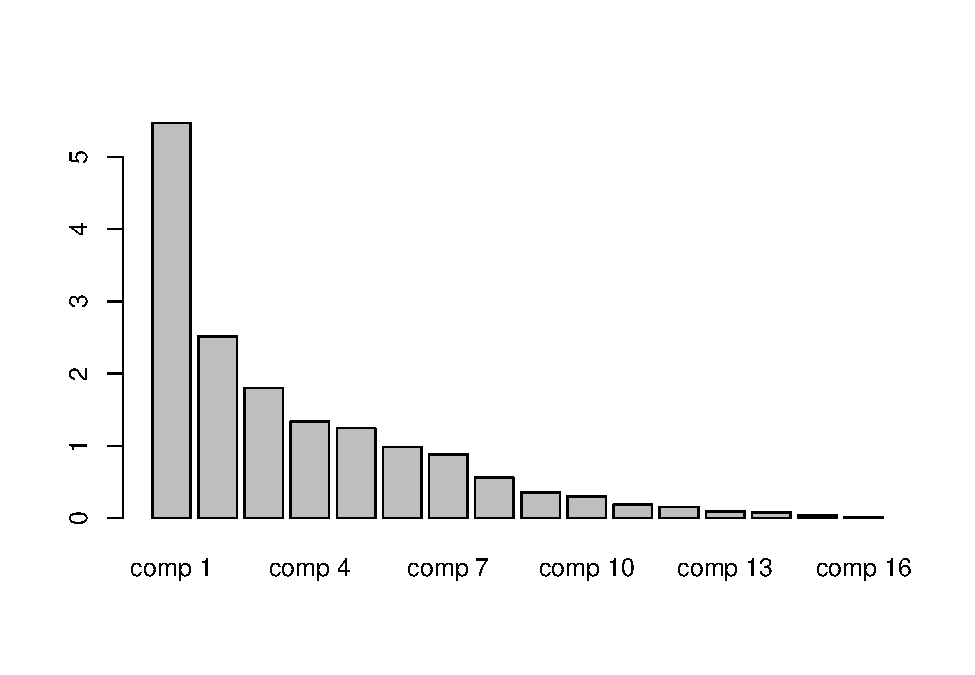
\includegraphics{salmon_files/figure-latex/unnamed-chunk-5-1.pdf}

Now, let's see what happens if we run the \textbf{plot.PCA} function to the \emph{res} object.

\begin{Shaded}
\begin{Highlighting}[]
\FunctionTok{plot.PCA}\NormalTok{(res,}\AttributeTok{choix=}\StringTok{"var"}\NormalTok{)}
\end{Highlighting}
\end{Shaded}

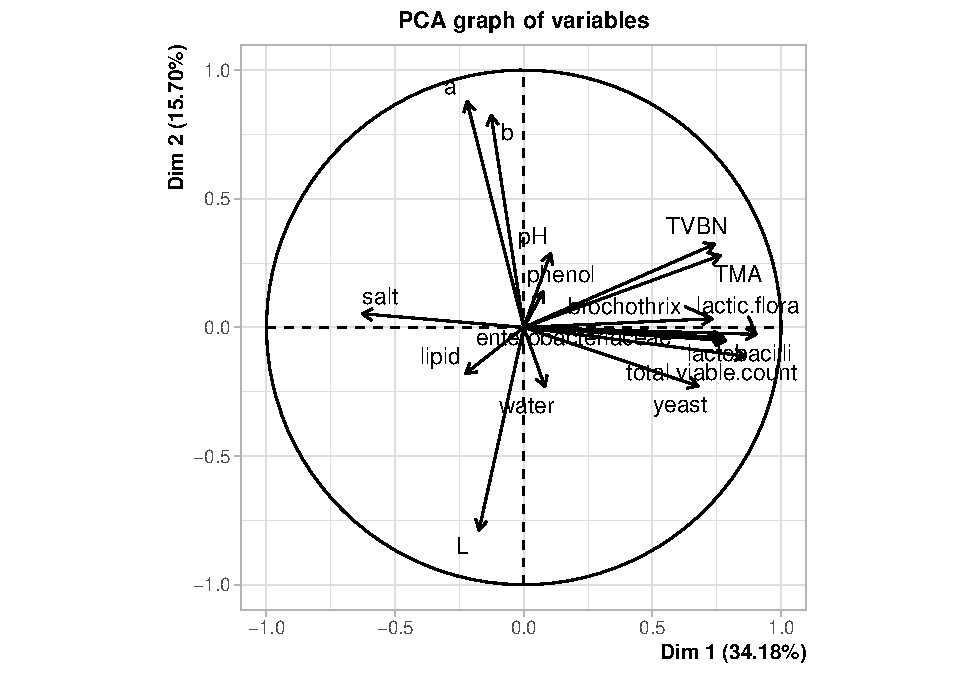
\includegraphics{salmon_files/figure-latex/unnamed-chunk-6-1.pdf}

\begin{Shaded}
\begin{Highlighting}[]
\FunctionTok{plot.PCA}\NormalTok{(res,}\AttributeTok{choix=}\StringTok{"ind"}\NormalTok{)}
\end{Highlighting}
\end{Shaded}

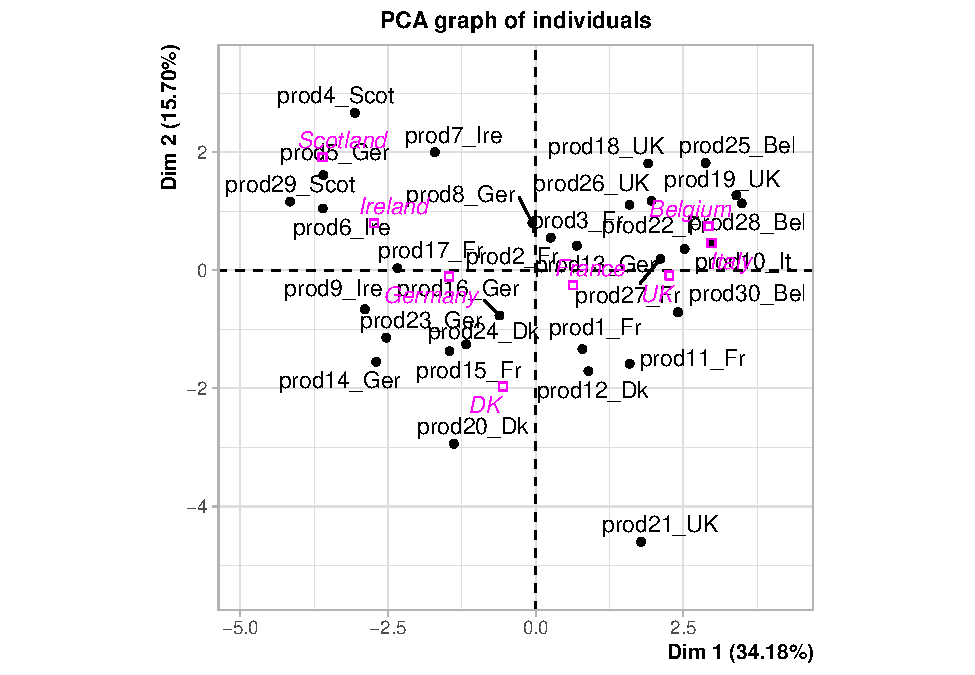
\includegraphics{salmon_files/figure-latex/unnamed-chunk-6-2.pdf}

\begin{Shaded}
\begin{Highlighting}[]
\FunctionTok{plot.PCA}\NormalTok{(res,}\AttributeTok{choix=}\StringTok{"ind"}\NormalTok{,}\AttributeTok{invisible=}\StringTok{"quali"}\NormalTok{)}
\end{Highlighting}
\end{Shaded}

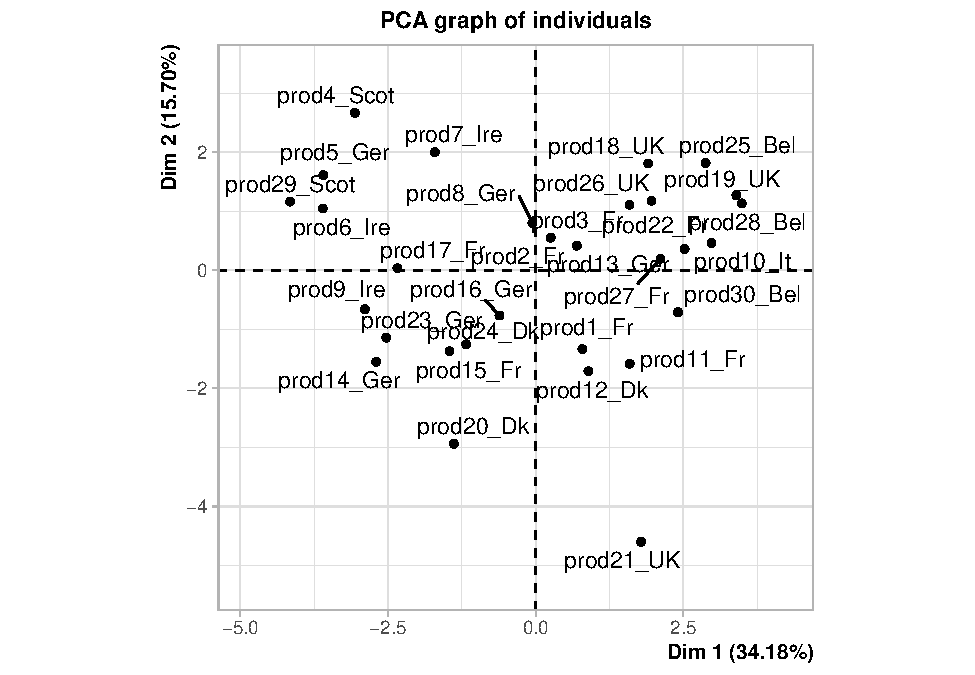
\includegraphics{salmon_files/figure-latex/unnamed-chunk-6-3.pdf}

As you can see, some news feature have been added to the \textbf{FactoMineR} package, notably the \emph{ggplot} type representation of the individuals and the variables. In this example, we can see how important \emph{supplementary} variables can be. We can also see how they can be represented, which is the case by default. Here, we projected the information on the origin of the smoked salmon. Look at the product 10, how do you think this product is salty?

Any questions about the concept of \emph{illustrative} variables? What do you think about the percentage associated with each axis?

Now that we know how to differentiate \emph{illustrative} or \emph{supplementary} variables from the \emph{active} ones, let's spend some time to interpret this PCA. As you know, the two graphical representations have to be interpreted jointly.

You may want to use the \textbf{dimdesc} function to get an interpretation of the axis.

\begin{Shaded}
\begin{Highlighting}[]
\NormalTok{resdim }\OtherTok{\textless{}{-}} \FunctionTok{dimdesc}\NormalTok{(res)}
\FunctionTok{names}\NormalTok{(resdim)}
\end{Highlighting}
\end{Shaded}

\begin{verbatim}
## [1] "Dim.1" "Dim.2" "Dim.3" "call"
\end{verbatim}

\begin{Shaded}
\begin{Highlighting}[]
\NormalTok{resdim}\SpecialCharTok{$}\NormalTok{Dim}\FloatTok{.1}
\end{Highlighting}
\end{Shaded}

\begin{verbatim}
## $quanti
##                    correlation      p.value
## lactic.flora         0.9027708 9.041485e-12
## total.viable.count   0.8608419 1.046362e-09
## lactobacilli         0.7850662 2.795050e-07
## enterobacteriaceae   0.7762724 4.619296e-07
## TMA                  0.7642286 8.873792e-07
## TVBN                 0.7421954 2.668420e-06
## brochothrix          0.7317464 4.332436e-06
## yeast                0.6773779 3.930677e-05
## salt                -0.6282864 2.011201e-04
## 
## $quali
##               R2      p.value
## origin 0.7348005 3.964817e-05
## 
## $category
##                  Estimate    p.value
## origin=Belgium   2.871677 0.02182312
## origin=UK        2.208683 0.03851838
## origin=Ireland  -2.788912 0.03325308
## origin=Scotland -3.662799 0.02354381
## 
## attr(,"class")
## [1] "condes" "list"
\end{verbatim}

Now, you can try to explore the dataset in a more dynamical manner. What is the difference between this,

\begin{Shaded}
\begin{Highlighting}[]
\FunctionTok{library}\NormalTok{(explor)}
\NormalTok{res }\OtherTok{\textless{}{-}} \FunctionTok{PCA}\NormalTok{(salmon\_car,}\AttributeTok{quali.sup=}\DecValTok{17}\NormalTok{,}\AttributeTok{graph=}\NormalTok{F)}
\FunctionTok{explor}\NormalTok{(res)}
\end{Highlighting}
\end{Shaded}

and this?

\begin{Shaded}
\begin{Highlighting}[]
\NormalTok{res }\OtherTok{\textless{}{-}} \FunctionTok{PCA}\NormalTok{(salmon\_car[,}\SpecialCharTok{{-}}\DecValTok{17}\NormalTok{],}\AttributeTok{graph=}\NormalTok{F)}
\FunctionTok{explor}\NormalTok{(res)}
\end{Highlighting}
\end{Shaded}

\textbf{Exercise. }
You can play with the different arguments of the \textbf{PCA} and the \textbf{plot.PCA} functions.

\textbf{Remark. }PCA, by extracting dimensions, can be seen as a method to summarize the data, or more precisely the relations amongst the variables of your dataset. Some people would say that by running a PCA you cluster variables into dimensions. It's very convenient, because you simplify your understanding by using a few dimensions instead of all the variables.
You could do the same thing with the individuals. Instead of reducing the complexity on your variables, you will reduce the complexity on the individuals.

\begin{Shaded}
\begin{Highlighting}[]
\NormalTok{reshcpc }\OtherTok{\textless{}{-}} \FunctionTok{HCPC}\NormalTok{(res,}\AttributeTok{nb.clust=}\DecValTok{3}\NormalTok{)}
\end{Highlighting}
\end{Shaded}

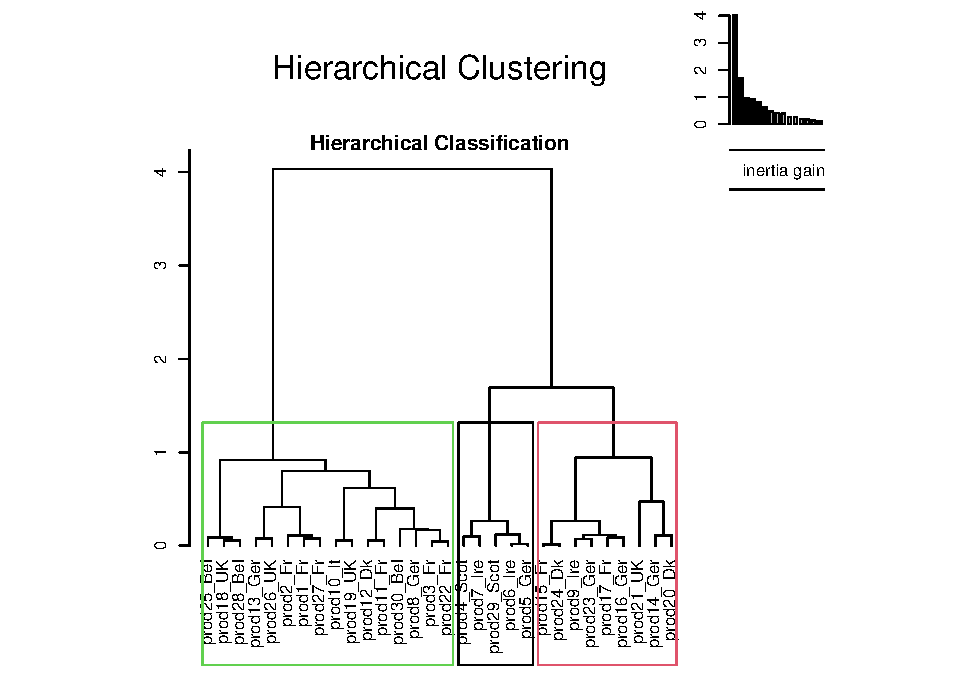
\includegraphics{salmon_files/figure-latex/unnamed-chunk-10-1.pdf} 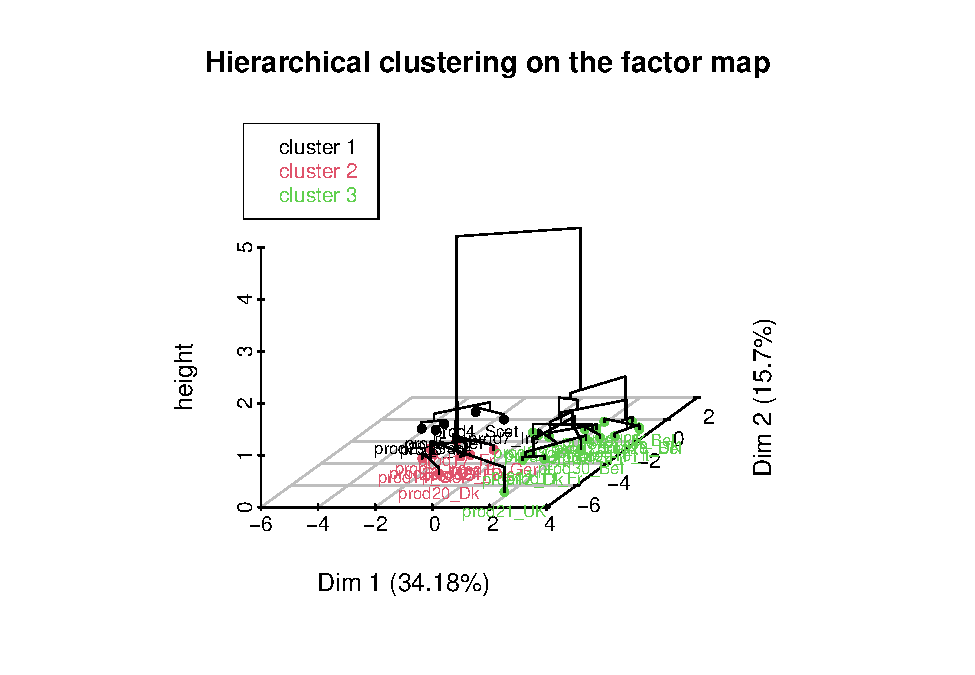
\includegraphics{salmon_files/figure-latex/unnamed-chunk-10-2.pdf} 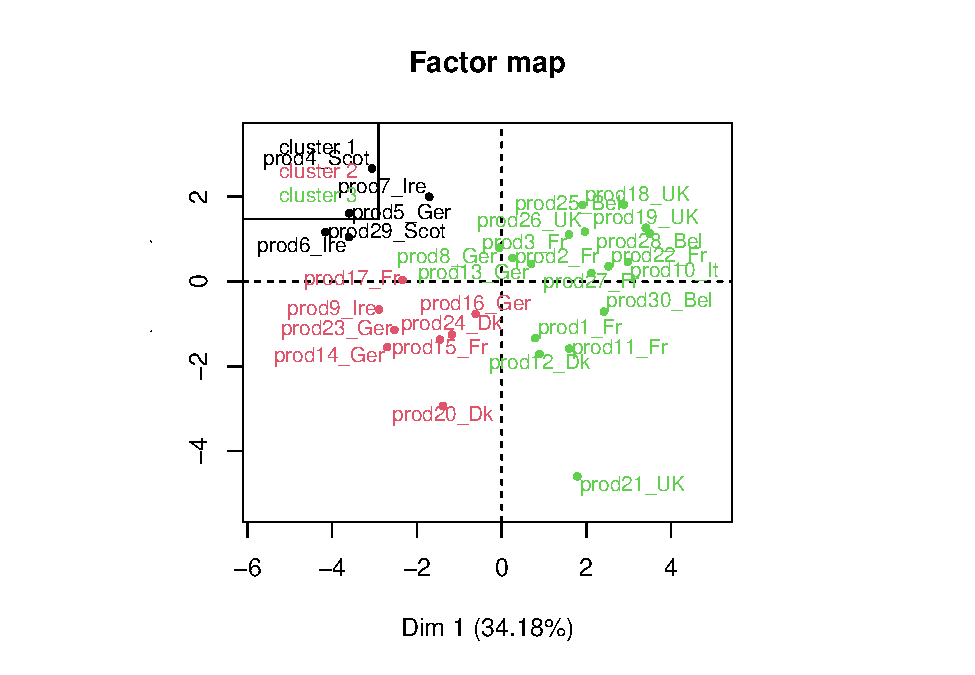
\includegraphics{salmon_files/figure-latex/unnamed-chunk-10-3.pdf}

\begin{Shaded}
\begin{Highlighting}[]
\FunctionTok{names}\NormalTok{(reshcpc)}
\end{Highlighting}
\end{Shaded}

\begin{verbatim}
## [1] "data.clust" "desc.var"   "desc.axes"  "desc.ind"   "call"
\end{verbatim}

\begin{Shaded}
\begin{Highlighting}[]
\FunctionTok{names}\NormalTok{(reshcpc}\SpecialCharTok{$}\NormalTok{desc.var)}
\end{Highlighting}
\end{Shaded}

\begin{verbatim}
## [1] "test.chi2"  "category"   "quanti.var" "quanti"     "call"
\end{verbatim}

\begin{Shaded}
\begin{Highlighting}[]
\FunctionTok{names}\NormalTok{(reshcpc}\SpecialCharTok{$}\NormalTok{desc.var}\SpecialCharTok{$}\NormalTok{quanti)}
\end{Highlighting}
\end{Shaded}

\begin{verbatim}
## [1] "1" "2" "3"
\end{verbatim}

\begin{Shaded}
\begin{Highlighting}[]
\NormalTok{reshcpc}\SpecialCharTok{$}\NormalTok{desc.var}\SpecialCharTok{$}\NormalTok{quanti}\SpecialCharTok{$}\StringTok{\textasciigrave{}}\AttributeTok{1}\StringTok{\textasciigrave{}}
\end{Highlighting}
\end{Shaded}

\begin{verbatim}
##                       v.test Mean in category  Overall mean sd in category
## b                   2.967108          1.23202 -3.333333e-06      1.1663873
## salt                2.404836          0.99856 -1.457168e-17      1.0973584
## a                   2.291474          0.95148 -3.700743e-18      0.4806493
## TMA                -2.099319         -0.87170  3.333333e-06      0.0000000
## yeast              -2.490229         -1.03400  3.333333e-06      0.0000000
## water              -2.519590         -1.04622 -1.000000e-05      0.5634578
## enterobacteriaceae -3.052957         -1.26770 -1.000000e-05      0.3944804
## lactic.flora       -3.077490         -1.27786  3.333333e-06      0.6164800
## total.viable.count -3.819886         -1.58612  6.666667e-06      0.9248322
##                    Overall sd      p.value
## b                   0.9999991 0.0030061550
## salt                1.0000064 0.0161797401
## a                   0.9999972 0.0219360319
## TMA                 1.0000099 0.0357888054
## yeast               0.9999921 0.0127660659
## water               1.0000067 0.0117491490
## enterobacteriaceae  1.0000148 0.0022659864
## lactic.flora        1.0000041 0.0020875189
## total.viable.count  1.0000033 0.0001335133
\end{verbatim}

\begin{Shaded}
\begin{Highlighting}[]
\NormalTok{reshcpc}\SpecialCharTok{$}\NormalTok{desc.var}\SpecialCharTok{$}\NormalTok{quanti}\SpecialCharTok{$}\StringTok{\textasciigrave{}}\AttributeTok{2}\StringTok{\textasciigrave{}}
\end{Highlighting}
\end{Shaded}

\begin{verbatim}
##                 v.test Mean in category  Overall mean sd in category Overall sd
## L             2.442596        0.7521750 -1.619075e-18      0.5146511  0.9999999
## water         2.241235        0.6901625 -1.000000e-05      0.9409535  1.0000067
## lactic.flora -2.264032       -0.6971875  3.333333e-06      0.7459357  1.0000041
## TMA          -2.291215       -0.7055625  3.333333e-06      0.2520950  1.0000099
## b            -2.309972       -0.7113375 -3.333333e-06      0.4989181  0.9999991
## TVBN         -2.396348       -0.7379375 -1.966020e-17      0.3225866  1.0000055
## brochothrix  -2.454675       -0.7559000 -5.551115e-18      0.0000000  1.0000069
## lactobacilli -2.903449       -0.8941125 -6.666667e-06      0.4452469  1.0000168
##                  p.value
## L            0.014582067
## water        0.025010865
## lactic.flora 0.023572148
## TMA          0.021950968
## b            0.020889703
## TVBN         0.016559366
## brochothrix  0.014101201
## lactobacilli 0.003690765
\end{verbatim}

\begin{Shaded}
\begin{Highlighting}[]
\NormalTok{reshcpc}\SpecialCharTok{$}\NormalTok{desc.var}\SpecialCharTok{$}\NormalTok{quanti}\SpecialCharTok{$}\StringTok{\textasciigrave{}}\AttributeTok{3}\StringTok{\textasciigrave{}}
\end{Highlighting}
\end{Shaded}

\begin{verbatim}
##                       v.test Mean in category  Overall mean sd in category
## lactic.flora        4.334916        0.7039353  3.333333e-06      0.4319264
## total.viable.count  4.055101        0.6585000  6.666667e-06      0.3942778
## lactobacilli        3.996881        0.6490412 -6.666667e-06      0.7748847
## enterobacteriaceae  3.794019        0.6160941 -1.000000e-05      0.6448174
## TMA                 3.623520        0.5884176  3.333333e-06      0.9648019
## yeast               3.602067        0.5849235  3.333333e-06      0.8154801
## brochothrix         3.559652        0.5780412 -5.551115e-18      0.9968236
## TVBN                3.303261        0.5364059 -1.966020e-17      1.0210896
## salt               -3.148943       -0.5113471 -1.457168e-17      0.6917277
##                    Overall sd      p.value
## lactic.flora        1.0000041 1.458157e-05
## total.viable.count  1.0000033 5.011257e-05
## lactobacilli        1.0000168 6.418262e-05
## enterobacteriaceae  1.0000148 1.482285e-04
## TMA                 1.0000099 2.906203e-04
## yeast               0.9999921 3.156966e-04
## brochothrix         1.0000069 3.713463e-04
## TVBN                1.0000055 9.556725e-04
## salt                1.0000064 1.638622e-03
\end{verbatim}

Instead of having 30 smoked salmons, we now have 3 groups of salmons: that's how we reduce the complexity of our problem.

Let's use a very interesting output of our \textbf{HCPC} function, and play with it.

\begin{Shaded}
\begin{Highlighting}[]
\FunctionTok{summary}\NormalTok{(reshcpc}\SpecialCharTok{$}\NormalTok{data.clust)}
\end{Highlighting}
\end{Shaded}

\begin{verbatim}
##      water              lipid                 TVBN              TMA            
##  Min.   :-1.69910   Min.   :-2.4628000   Min.   :-1.1623   Min.   :-0.8717000  
##  1st Qu.:-0.85198   1st Qu.:-0.4259750   1st Qu.:-0.7629   1st Qu.:-0.8717000  
##  Median :-0.07435   Median : 0.2159000   Median :-0.3635   Median :-0.2757000  
##  Mean   :-0.00001   Mean   : 0.0000067   Mean   : 0.0000   Mean   : 0.0000033  
##  3rd Qu.: 0.47713   3rd Qu.: 0.5763000   3rd Qu.: 0.4354   3rd Qu.: 0.5439000  
##  Max.   : 2.02730   Max.   : 1.6251000   Max.   : 2.6322   Max.   : 2.4065000  
##                                                                                
##       salt             phenol               pH             total.viable.count  
##  Min.   :-2.0049   Min.   :-1.20730   Min.   :-1.7733000   Min.   :-2.5977000  
##  1st Qu.:-0.6115   1st Qu.:-0.65633   1st Qu.:-0.8617500   1st Qu.:-0.3530250  
##  Median : 0.0077   Median :-0.29985   Median :-0.0331500   Median : 0.2699000  
##  Mean   : 0.0000   Mean   : 0.00001   Mean   :-0.0000067   Mean   : 0.0000067  
##  3rd Qu.: 0.3174   3rd Qu.: 0.40010   3rd Qu.: 0.8368750   3rd Qu.: 0.8187750  
##  Max.   : 2.4848   Max.   : 3.45930   Max.   : 2.0384000   Max.   : 1.1384000  
##                                                                                
##   lactic.flora         lactobacilli         brochothrix     
##  Min.   :-1.5861000   Min.   :-1.0624000   Min.   :-0.7559  
##  1st Qu.:-0.4710500   1st Qu.:-1.0624000   1st Qu.:-0.7559  
##  Median : 0.3886500   Median : 0.2064500   Median :-0.7559  
##  Mean   : 0.0000033   Mean   :-0.0000067   Mean   : 0.0000  
##  3rd Qu.: 0.8312750   3rd Qu.: 0.9333500   3rd Qu.: 0.8192  
##  Max.   : 1.5327000   Max.   : 1.9639000   Max.   : 2.4632  
##                                                             
##      yeast            enterobacteriaceae       L                 a          
##  Min.   :-1.0340000   Min.   :-1.57930   Min.   :-1.8353   Min.   :-3.9939  
##  1st Qu.:-1.0340000   1st Qu.:-0.65815   1st Qu.:-0.8034   1st Qu.:-0.4152  
##  Median : 0.2608000   Median : 0.04190   Median : 0.1441   Median : 0.2868  
##  Mean   : 0.0000033   Mean   :-0.00001   Mean   : 0.0000   Mean   : 0.0000  
##  3rd Qu.: 0.7537750   3rd Qu.: 0.79060   3rd Qu.: 0.5455   3rd Qu.: 0.5362  
##  Max.   : 2.1072000   Max.   : 1.64720   Max.   : 2.5982   Max.   : 1.7439  
##                                                                             
##        b                 origin  clust 
##  Min.   :-1.827700   France :8   1: 5  
##  1st Qu.:-0.577750   Germany:6   2: 8  
##  Median : 0.073650   UK     :4   3:17  
##  Mean   :-0.000003   Belgium:3         
##  3rd Qu.: 0.388475   DK     :3         
##  Max.   : 3.323600   Ireland:3         
##                      (Other):3
\end{verbatim}

\begin{Shaded}
\begin{Highlighting}[]
\NormalTok{res }\OtherTok{\textless{}{-}} \FunctionTok{PCA}\NormalTok{(reshcpc}\SpecialCharTok{$}\NormalTok{data.clust,}\AttributeTok{quali.sup=}\FunctionTok{c}\NormalTok{(}\DecValTok{17}\NormalTok{,}\DecValTok{18}\NormalTok{),}\AttributeTok{graph=}\NormalTok{F)}
\FunctionTok{plot.PCA}\NormalTok{(res,}\AttributeTok{choix=}\StringTok{"var"}\NormalTok{,}\AttributeTok{graph.type =} \StringTok{"classic"}\NormalTok{)}
\end{Highlighting}
\end{Shaded}

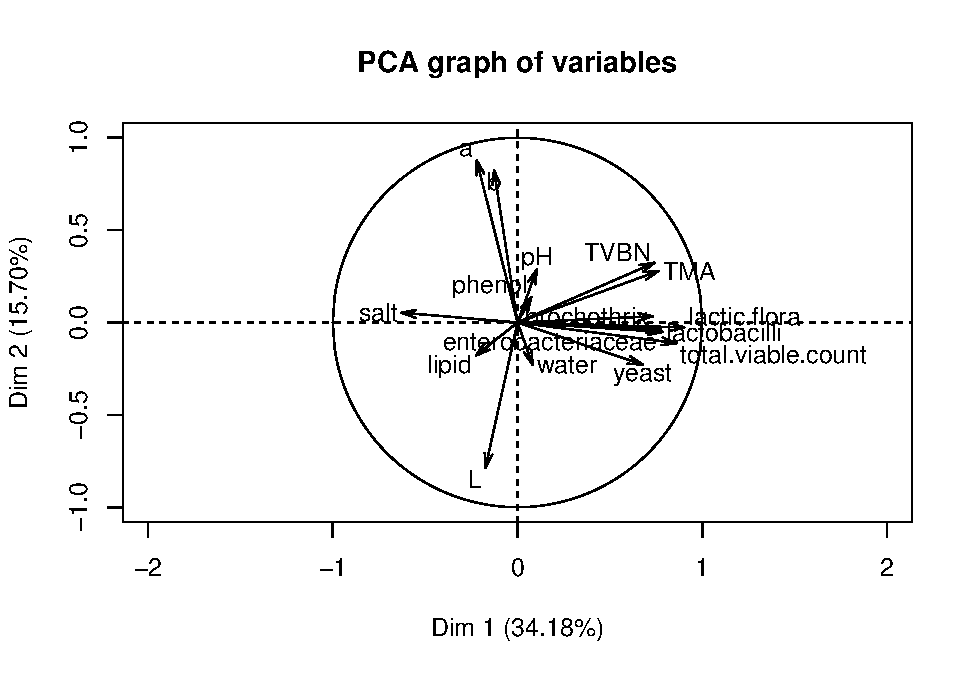
\includegraphics{salmon_files/figure-latex/unnamed-chunk-11-1.pdf}

\begin{Shaded}
\begin{Highlighting}[]
\FunctionTok{plot.PCA}\NormalTok{(res,}\AttributeTok{choix=}\StringTok{"var"}\NormalTok{,}\AttributeTok{graph.type =} \StringTok{"ggplot"}\NormalTok{)}
\end{Highlighting}
\end{Shaded}

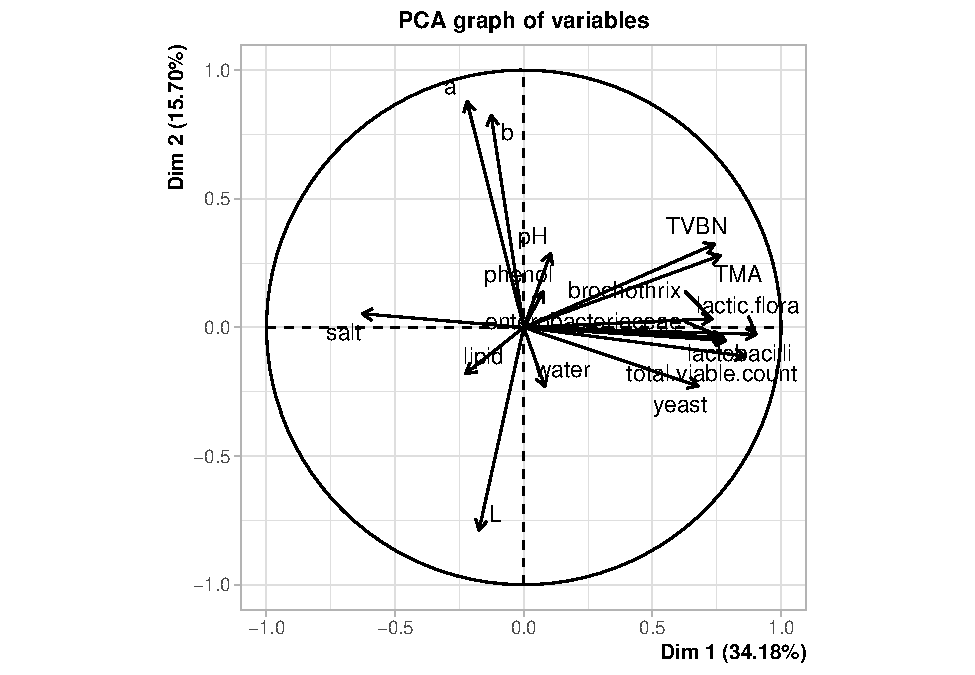
\includegraphics{salmon_files/figure-latex/unnamed-chunk-11-2.pdf}

\begin{Shaded}
\begin{Highlighting}[]
\FunctionTok{plot.PCA}\NormalTok{(res,}\AttributeTok{choix=}\StringTok{"ind"}\NormalTok{,}\AttributeTok{invisible=}\StringTok{"quali"}\NormalTok{,}\AttributeTok{habillage =} \DecValTok{17}\NormalTok{)}
\end{Highlighting}
\end{Shaded}

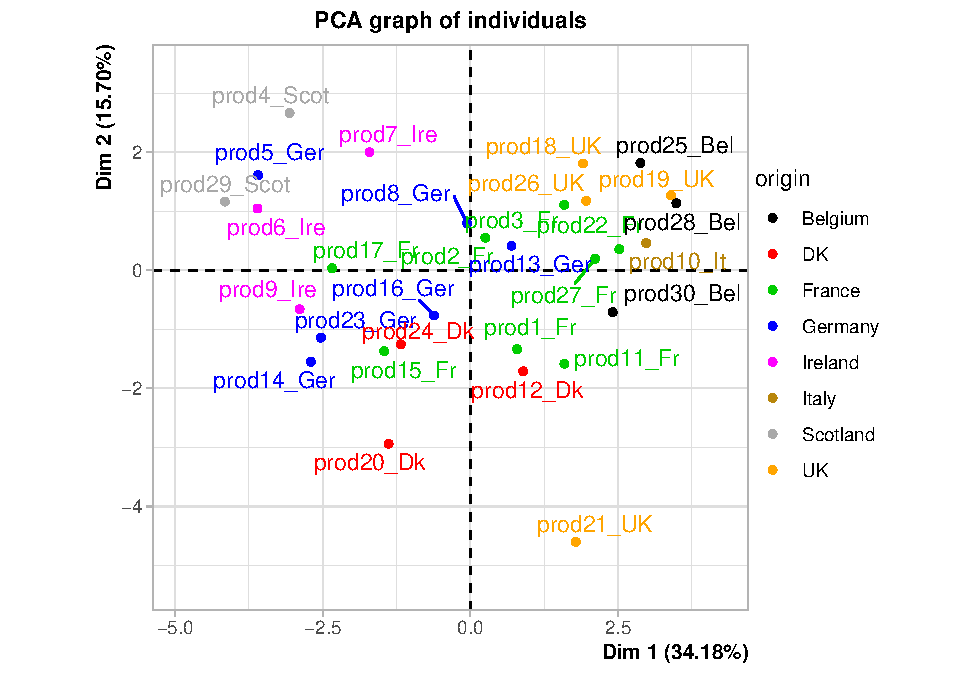
\includegraphics{salmon_files/figure-latex/unnamed-chunk-11-3.pdf}

\begin{Shaded}
\begin{Highlighting}[]
\FunctionTok{plot.PCA}\NormalTok{(res,}\AttributeTok{choix=}\StringTok{"ind"}\NormalTok{,}\AttributeTok{invisible=}\StringTok{"quali"}\NormalTok{,}\AttributeTok{habillage =} \DecValTok{18}\NormalTok{)}
\end{Highlighting}
\end{Shaded}

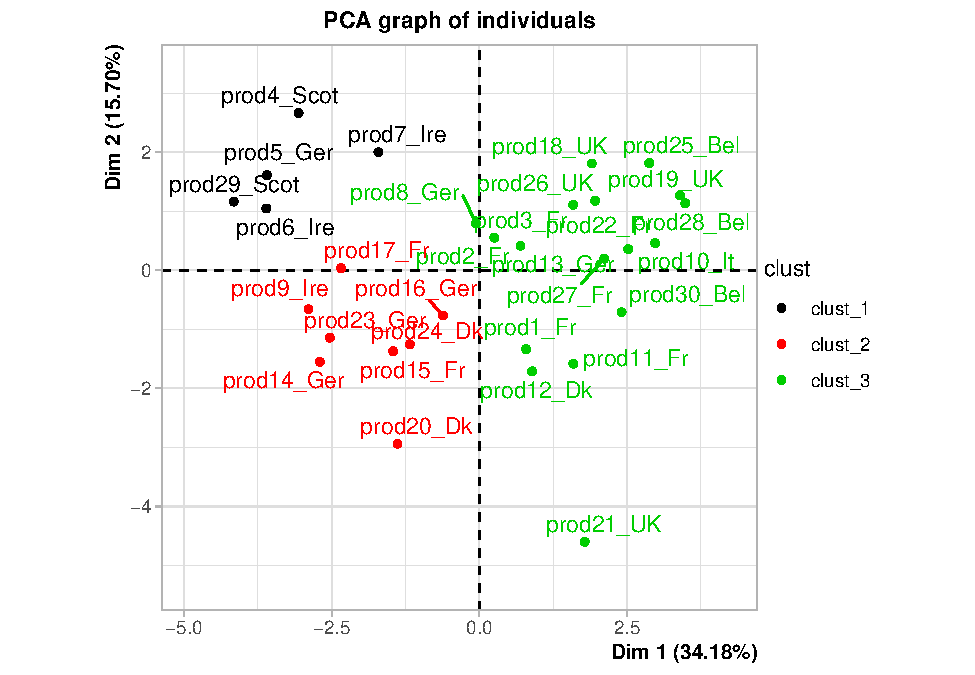
\includegraphics{salmon_files/figure-latex/unnamed-chunk-11-4.pdf}

\begin{Shaded}
\begin{Highlighting}[]
\FunctionTok{plot.PCA}\NormalTok{(res,}\AttributeTok{choix=}\StringTok{"ind"}\NormalTok{,}\AttributeTok{invisible=}\StringTok{"ind"}\NormalTok{)}
\end{Highlighting}
\end{Shaded}

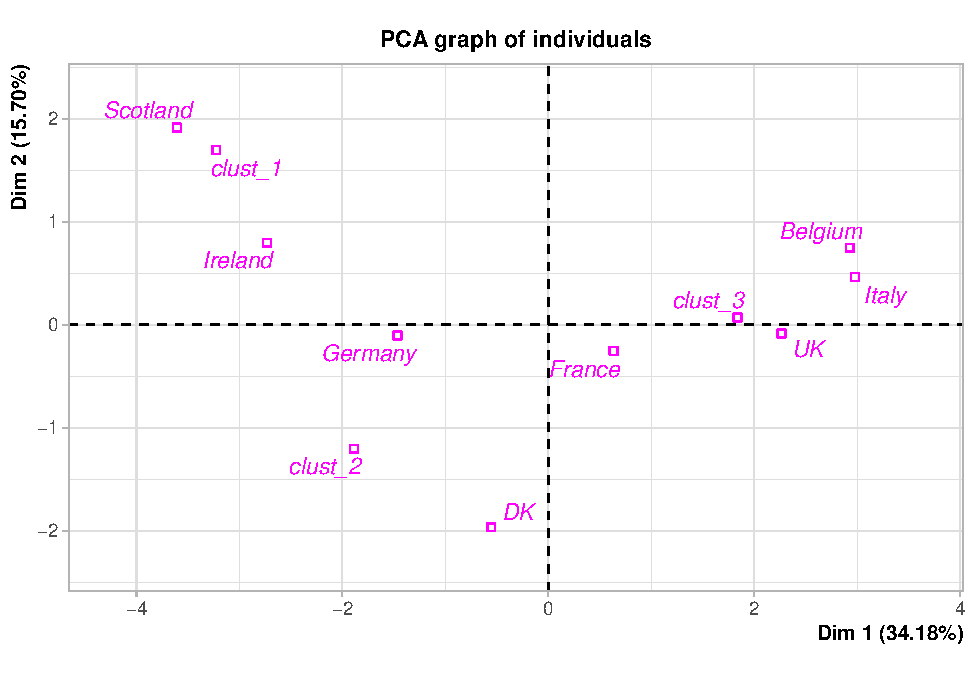
\includegraphics{salmon_files/figure-latex/unnamed-chunk-11-5.pdf}

\begin{Shaded}
\begin{Highlighting}[]
\FunctionTok{plot}\NormalTok{(res,}\AttributeTok{habillage=}\StringTok{"salt"}\NormalTok{,}\AttributeTok{ggoptions=}\FunctionTok{list}\NormalTok{(}\AttributeTok{low.col.quanti=}\StringTok{"grey90"}\NormalTok{,}\AttributeTok{high.col.quanti=}\StringTok{"grey10"}\NormalTok{),}
\AttributeTok{legend=}\FunctionTok{list}\NormalTok{(}\AttributeTok{x=}\StringTok{"bottom"}\NormalTok{),}\AttributeTok{invisible =} \StringTok{"quali"}\NormalTok{)}
\end{Highlighting}
\end{Shaded}

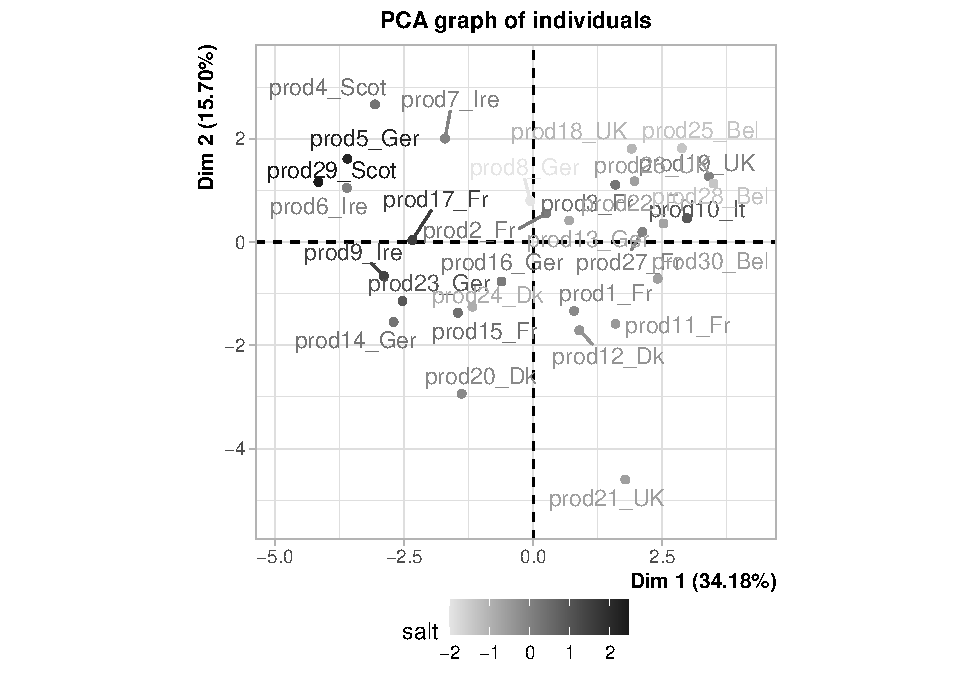
\includegraphics{salmon_files/figure-latex/unnamed-chunk-11-6.pdf}

\textbf{Exercise. }This exercise is very important as it presents two very useful functions of the \textbf{FactoMineR} package.

\begin{Shaded}
\begin{Highlighting}[]
\FunctionTok{descfreq}\NormalTok{(}\FunctionTok{table}\NormalTok{(reshcpc}\SpecialCharTok{$}\NormalTok{data.clust}\SpecialCharTok{$}\NormalTok{clust,reshcpc}\SpecialCharTok{$}\NormalTok{data.clust}\SpecialCharTok{$}\NormalTok{origin))}
\FunctionTok{catdes}\NormalTok{(reshcpc}\SpecialCharTok{$}\NormalTok{data.clust,}\AttributeTok{num.var=}\DecValTok{18}\NormalTok{)}
\end{Highlighting}
\end{Shaded}

To understand the code, you should first run this:

\begin{Shaded}
\begin{Highlighting}[]
\FunctionTok{table}\NormalTok{(reshcpc}\SpecialCharTok{$}\NormalTok{data.clust}\SpecialCharTok{$}\NormalTok{clust,reshcpc}\SpecialCharTok{$}\NormalTok{data.clust}\SpecialCharTok{$}\NormalTok{origin)}
\FunctionTok{colnames}\NormalTok{(reshcpc}\SpecialCharTok{$}\NormalTok{data.clust)}
\end{Highlighting}
\end{Shaded}

\textbf{Exercise. }Please, provide a description of the French salmons.

\hypertarget{understanding-the-products-from-a-hedonic-point-of-view}{%
\section{Understanding the products from a hedonic point of view}\label{understanding-the-products-from-a-hedonic-point-of-view}}

This part will be more easy than the first one, now that you know how to run R functions. The only complicated thing is the dataset we're going to use.

\begin{Shaded}
\begin{Highlighting}[]
\NormalTok{salmon\_hedo\_conso }\OtherTok{\textless{}{-}} \FunctionTok{read.delim2}\NormalTok{(}\StringTok{"salmon\_hedo\_conso.txt"}\NormalTok{, }\AttributeTok{header=}\ConstantTok{TRUE}\NormalTok{, }\AttributeTok{row.names=}\DecValTok{1}\NormalTok{, }\AttributeTok{comment.char=}\StringTok{"\#"}\NormalTok{,}\AttributeTok{dec=}\StringTok{","}\NormalTok{,}\AttributeTok{stringsAsFactors=}\ConstantTok{TRUE}\NormalTok{)}
\FunctionTok{colnames}\NormalTok{(salmon\_hedo\_conso)}
\end{Highlighting}
\end{Shaded}

\begin{verbatim}
##   [1] "IKIDEN"                  "Country"                
##   [3] "prod1_Fr"                "prod2_Fr"               
##   [5] "prod3_Fr"                "prod4_Scot"             
##   [7] "prod5_Ger"               "prod6_Ire"              
##   [9] "prod7_Ire"               "prod8_Ger"              
##  [11] "prod9_Ire"               "prod10_It"              
##  [13] "prod11_Fr"               "prod12_Dk"              
##  [15] "prod13_Ger"              "prod14_Ger"             
##  [17] "prod15_Fr"               "prod16_Ger"             
##  [19] "prod17_Fr"               "prod18_UK"              
##  [21] "prod19_UK"               "prod20_Dk"              
##  [23] "prod21_UK"               "prod22_Fr"              
##  [25] "prod23_Ger"              "prod24_Dk"              
##  [27] "prod25_Bel"              "prod26_UK"              
##  [29] "prod27_Fr"               "prod28_Bel"             
##  [31] "prod29_Scot"             "prod30_Bel"             
##  [33] "Who"                     "Frequence"              
##  [35] "When"                    "Taste"                  
##  [37] "Healthy"                 "Pleasure"               
##  [39] "No.preparation"          "Ways"                   
##  [41] "Guest"                   "Authentic"              
##  [43] "Not.expensive"           "Supermarket"            
##  [45] "Deli"                    "Caterer"                
##  [47] "Fish.shop"               "Market"                 
##  [49] "Mobile.van"              "Everyday"               
##  [51] "Special"                 "Day.snack"              
##  [53] "Evening.snack"           "Aperitif"               
##  [55] "Starter"                 "Salad"                  
##  [57] "Cooked.meal"             "Sandwich"               
##  [59] "Main"                    "Vegetable"              
##  [61] "Lemon"                   "Bread..butter"          
##  [63] "Lemon..bread..butter"    "C..fraiche"             
##  [65] "C..fraiche.with.herbs"   "Fresh.cheese"           
##  [67] "Fresh.cheese.with.herbs" "Shallots"               
##  [69] "Mustard"                 "Butter"                 
##  [71] "Black.pepper"            "Horseradish"            
##  [73] "Scottish"                "Norwegian"              
##  [75] "Atlantic"                "Irish"                  
##  [77] "Wild"                    "Do.not.know"            
##  [79] "Colour"                  "Price"                  
##  [81] "Origin"                  "Brand"                  
##  [83] "Advertising"             "Glossiness"             
##  [85] "Packaging"               "Labelling.information"  
##  [87] "Number.slices"           "Weight"                 
##  [89] "Use.by.date"             "Usual.brand"            
##  [91] "Appetising"              "Firm"                   
##  [93] "Regular"                 "Nice.colour"            
##  [95] "Nice.odour"              "Smooth.texture"         
##  [97] "Firm.texture"            "Greasy.mouth"           
##  [99] "Characteristic.taste"    "Not.too.salty"
\end{verbatim}

\begin{Shaded}
\begin{Highlighting}[]
\NormalTok{salmon\_hedo }\OtherTok{\textless{}{-}}\NormalTok{ salmon\_hedo\_conso[,}\DecValTok{3}\SpecialCharTok{:}\DecValTok{32}\NormalTok{]}
\FunctionTok{head}\NormalTok{(salmon\_hedo)}
\end{Highlighting}
\end{Shaded}

\begin{verbatim}
##          prod1_Fr prod2_Fr prod3_Fr prod4_Scot prod5_Ger prod6_Ire prod7_Ire
## 5101Lyon   0.5433   0.5433  -0.0187     0.5433    0.5433   -0.0187    1.1054
## 5102Lyon   0.4685  -0.3123   0.4685     0.4685    1.2494   -1.0932   -0.3123
## 5103Lyon   0.4354   1.3683  -0.9641     0.4354    1.3683   -0.4976    0.4354
## 5106Lyon   1.6920   1.6920   0.6004     1.1462    0.6004   -0.4912   -1.0371
## 5107Lyon   0.6167  -0.2056   0.2056    -0.6167   -1.4389    0.6167    0.6167
## 5108Lyon  -0.0165   0.9714  -1.9922     0.9714   -1.0043    0.9714   -0.5104
##          prod8_Ger prod9_Ire prod10_It prod11_Fr prod12_Dk prod13_Ger
## 5101Lyon   -0.5808    0.5433   -0.5808   -0.0187   -2.8290     0.5433
## 5102Lyon    1.2494    0.4685   -0.3123    1.2494    0.4685    -0.3123
## 5103Lyon   -0.4976    0.4354   -0.9641   -0.9641   -0.0311    -0.0311
## 5106Lyon   -1.5829    0.6004    0.0546   -0.4912    0.0546    -1.5829
## 5107Lyon    0.2056    1.0278    0.6167   -0.6167    0.6167     1.0278
## 5108Lyon    1.4653    0.4775   -0.5104    1.4653    0.4775     0.4775
##          prod14_Ger prod15_Fr prod16_Ger prod17_Fr prod18_UK prod19_UK
## 5101Lyon    -1.7049   -1.7049    -1.1428    1.6674   -0.0187    0.5433
## 5102Lyon     1.2494   -2.6550     1.2494   -1.8741   -1.0932    0.4685
## 5103Lyon    -0.9641    0.9019    -2.3635    0.4354   -1.8970    0.4354
## 5106Lyon    -1.0371    0.6004     0.0546   -1.0371   -1.5829   -1.0371
## 5107Lyon     0.2056   -1.8500    -0.6167    0.6167    0.6167    1.0278
## 5108Lyon     0.9714    0.4775    -0.0165    0.4775   -1.9922   -1.4983
##          prod20_Dk prod21_UK prod22_Fr prod23_Ger prod24_Dk prod25_Bel
## 5101Lyon   -0.5808    1.1054    1.6674    -0.5808    0.5433     0.5433
## 5102Lyon   -1.0932    0.4685    1.2494    -1.0932   -1.0932     0.4685
## 5103Lyon    0.9019    0.4354   -1.4305     0.4354    0.9019     1.3683
## 5106Lyon   -0.4912    1.6920    0.0546     1.1462    0.6004    -0.4912
## 5107Lyon    1.4389   -1.4389    1.0278     1.4389   -1.8500    -1.0278
## 5108Lyon   -0.5104   -0.5104   -0.5104     1.4653   -1.0043    -0.0165
##          prod26_UK prod27_Fr prod28_Bel prod29_Scot prod30_Bel
## 5101Lyon   -0.0187   -1.1428    -0.5808      1.1054    -0.0187
## 5102Lyon   -0.3123   -0.3123    -0.3123      1.2494    -0.3123
## 5103Lyon   -0.4976   -0.0311     1.3683      0.9019    -1.4305
## 5106Lyon    0.0546   -1.0371    -0.4912      0.0546     1.6920
## 5107Lyon   -0.6167   -1.0278    -1.8500      0.6167     0.6167
## 5108Lyon   -1.0043   -0.0165    -1.4983      0.9714     0.9714
\end{verbatim}

\begin{Shaded}
\begin{Highlighting}[]
\FunctionTok{summary}\NormalTok{(salmon\_hedo)}
\end{Highlighting}
\end{Shaded}

\begin{verbatim}
##     prod1_Fr          prod2_Fr           prod3_Fr         prod4_Scot     
##  Min.   :-2.1360   Min.   :-3.72220   Min.   :-2.7302   Min.   :-2.1235  
##  1st Qu.:-0.3774   1st Qu.:-0.68700   1st Qu.:-0.9501   1st Qu.:-0.3297  
##  Median : 0.3375   Median : 0.13755   Median :-0.1479   Median : 0.3313  
##  Mean   : 0.2452   Mean   : 0.04939   Mean   :-0.1508   Mean   : 0.2508  
##  3rd Qu.: 0.9498   3rd Qu.: 0.86118   3rd Qu.: 0.6817   3rd Qu.: 0.9079  
##  Max.   : 2.9666   Max.   : 2.26040   Max.   : 2.2639   Max.   : 2.6550  
##    prod5_Ger         prod6_Ire         prod7_Ire         prod8_Ger       
##  Min.   :-2.5337   Min.   :-2.4287   Min.   :-3.1814   Min.   :-2.88000  
##  1st Qu.:-0.4006   1st Qu.:-0.5253   1st Qu.:-0.9135   1st Qu.:-0.85177  
##  Median : 0.4531   Median : 0.2530   Median :-0.1530   Median : 0.08645  
##  Mean   : 0.2866   Mean   : 0.1304   Mean   :-0.1728   Mean   :-0.02451  
##  3rd Qu.: 1.0272   3rd Qu.: 0.8346   3rd Qu.: 0.5827   3rd Qu.: 0.83683  
##  Max.   : 2.2748   Max.   : 2.3256   Max.   : 2.1494   Max.   : 2.47150  
##    prod9_Ire         prod10_It         prod11_Fr           prod12_Dk       
##  Min.   :-5.3852   Min.   :-3.1743   Min.   :-3.230300   Min.   :-3.33710  
##  1st Qu.:-0.4916   1st Qu.:-1.1219   1st Qu.:-0.753850   1st Qu.:-0.80768  
##  Median : 0.3034   Median :-0.3754   Median : 0.084350   Median : 0.11725  
##  Mean   : 0.1769   Mean   :-0.3395   Mean   :-0.005055   Mean   : 0.01955  
##  3rd Qu.: 0.9271   3rd Qu.: 0.4337   3rd Qu.: 0.777050   3rd Qu.: 0.86140  
##  Max.   : 2.1506   Max.   : 2.6033   Max.   : 2.221300   Max.   : 2.23290  
##    prod13_Ger        prod14_Ger          prod15_Fr          prod16_Ger     
##  Min.   :-2.3088   Min.   :-2.268400   Min.   :-2.99480   Min.   :-2.8800  
##  1st Qu.:-0.5555   1st Qu.:-0.804800   1st Qu.:-0.79033   1st Qu.:-1.0654  
##  Median : 0.2975   Median : 0.082850   Median : 0.05575   Median :-0.1009  
##  Mean   : 0.1776   Mean   : 0.001343   Mean   :-0.03593   Mean   :-0.1462  
##  3rd Qu.: 0.9225   3rd Qu.: 0.786775   3rd Qu.: 0.75270   3rd Qu.: 0.7339  
##  Max.   : 2.5355   Max.   : 2.171200   Max.   : 2.92530   Max.   : 2.5916  
##    prod17_Fr         prod18_UK         prod19_UK          prod20_Dk      
##  Min.   :-3.1593   Min.   :-4.7616   Min.   :-3.02240   Min.   :-2.9866  
##  1st Qu.:-0.5062   1st Qu.:-1.0661   1st Qu.:-0.96808   1st Qu.:-1.0533  
##  Median : 0.3222   Median :-0.0846   Median : 0.01865   Median :-0.2525  
##  Mean   : 0.2043   Mean   :-0.1246   Mean   :-0.06525   Mean   :-0.2454  
##  3rd Qu.: 0.9367   3rd Qu.: 0.8095   3rd Qu.: 0.83368   3rd Qu.: 0.5702  
##  Max.   : 2.2967   Max.   : 2.4062   Max.   : 2.17190   Max.   : 2.2533  
##    prod21_UK         prod22_Fr         prod23_Ger        prod24_Dk      
##  Min.   :-3.2295   Min.   :-2.5573   Min.   :-2.7796   Min.   :-2.9200  
##  1st Qu.:-1.3330   1st Qu.:-0.3786   1st Qu.:-0.5193   1st Qu.:-0.9318  
##  Median :-0.6263   Median : 0.4188   Median : 0.3100   Median :-0.1135  
##  Mean   :-0.4891   Mean   : 0.2796   Mean   : 0.2141   Mean   :-0.1635  
##  3rd Qu.: 0.3882   3rd Qu.: 0.9916   3rd Qu.: 0.9432   3rd Qu.: 0.5862  
##  Max.   : 2.2749   Max.   : 2.9192   Max.   : 2.2837   Max.   : 2.1106  
##    prod25_Bel        prod26_UK           prod27_Fr         prod28_Bel      
##  Min.   :-3.7989   Min.   :-3.246900   Min.   :-3.4338   Min.   :-3.86570  
##  1st Qu.:-1.0892   1st Qu.:-0.775475   1st Qu.:-0.5337   1st Qu.:-0.92065  
##  Median :-0.2366   Median : 0.023550   Median : 0.2627   Median :-0.07275  
##  Mean   :-0.2261   Mean   : 0.003309   Mean   : 0.1451   Mean   :-0.08774  
##  3rd Qu.: 0.6520   3rd Qu.: 0.835625   3rd Qu.: 0.9037   3rd Qu.: 0.78080  
##  Max.   : 2.5281   Max.   : 2.335100   Max.   : 2.1495   Max.   : 2.26810  
##   prod29_Scot         prod30_Bel       
##  Min.   :-2.85220   Min.   :-3.098800  
##  1st Qu.:-0.65350   1st Qu.:-0.835475  
##  Median : 0.14970   Median : 0.059250  
##  Mean   : 0.08247   Mean   : 0.009738  
##  3rd Qu.: 0.85493   3rd Qu.: 0.908800  
##  Max.   : 2.08720   Max.   : 2.184200
\end{verbatim}

\textbf{Exercise. }What do you think you have in the dataset \emph{salmon\_hedo}?

Let's run the following code:

\begin{Shaded}
\begin{Highlighting}[]
\NormalTok{res }\OtherTok{\textless{}{-}} \FunctionTok{PCA}\NormalTok{(}\FunctionTok{t}\NormalTok{(salmon\_hedo),}\AttributeTok{graph=}\NormalTok{F)}
\FunctionTok{plot.PCA}\NormalTok{(res,}\AttributeTok{choix=}\StringTok{"var"}\NormalTok{)}
\end{Highlighting}
\end{Shaded}

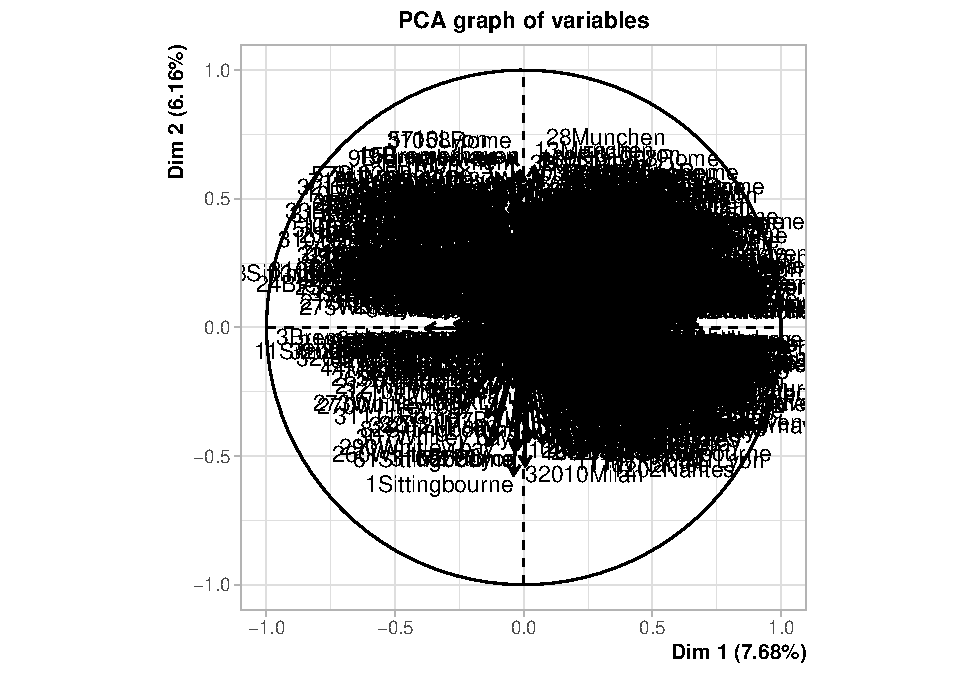
\includegraphics{salmon_files/figure-latex/unnamed-chunk-15-1.pdf}

\begin{Shaded}
\begin{Highlighting}[]
\FunctionTok{plot.PCA}\NormalTok{(res,}\AttributeTok{choix=}\StringTok{"ind"}\NormalTok{)}
\end{Highlighting}
\end{Shaded}

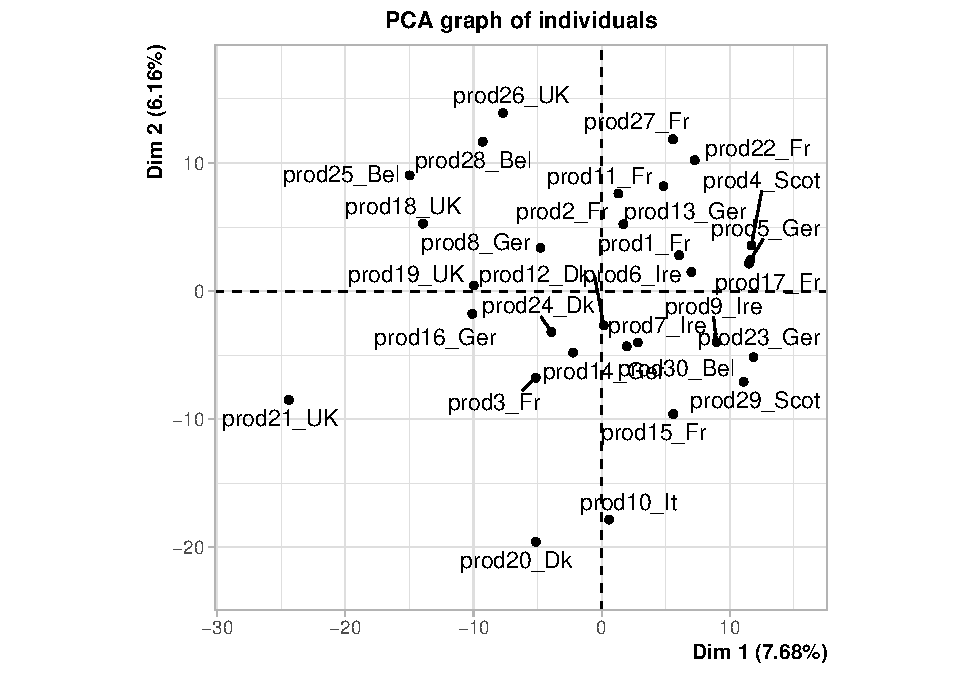
\includegraphics{salmon_files/figure-latex/unnamed-chunk-15-2.pdf}

Here, we've transposed the dataset, which means that the statistical individuals are now the smoked salmons, and not the consumers any more: salmons are described by the preferences provided by the consumers.

\textbf{Exercise. }How can you get a better representation of the variables?

\hypertarget{understanding-the-data-from-a-consumer-perspective}{%
\chapter{Understanding the data from a consumer perspective}\label{understanding-the-data-from-a-consumer-perspective}}

\hypertarget{playing-with-r-and-the-data}{%
\section{Playing with R and the data}\label{playing-with-r-and-the-data}}

In this part, the analyses are not going to be too complicated, but you will see that data manipulation and visualization is not simple when you deal with categorical variables.
Please install and load the two following packages.

\begin{Shaded}
\begin{Highlighting}[]
\FunctionTok{install.packages}\NormalTok{(}\StringTok{"questionr"}\NormalTok{)}
\FunctionTok{install.packages}\NormalTok{(}\StringTok{"dataMaid"}\NormalTok{)}
\end{Highlighting}
\end{Shaded}

\begin{Shaded}
\begin{Highlighting}[]
\FunctionTok{library}\NormalTok{(questionr)}
\FunctionTok{library}\NormalTok{(dataMaid)}
\end{Highlighting}
\end{Shaded}

\textbf{Exercise. }Comment on the different ways of describing the data.

\begin{Shaded}
\begin{Highlighting}[]
\FunctionTok{summary}\NormalTok{(salmon\_hedo\_conso)}
\FunctionTok{str}\NormalTok{(salmon\_hedo\_conso)}
\FunctionTok{describe}\NormalTok{(salmon\_hedo\_conso)}
\FunctionTok{describe}\NormalTok{(salmon\_hedo\_conso[,}\DecValTok{32}\SpecialCharTok{:}\DecValTok{40}\NormalTok{])}
\end{Highlighting}
\end{Shaded}

In the following part, we're going to change the names of the variables as well as their labels, to change the order of the levels of a given factor of interest as well as their value ; finally, we're going to plot a categorical variable, in a simple way and in a more complicated way.

\begin{Shaded}
\begin{Highlighting}[]
\CommentTok{\#Manipulating data}
\CommentTok{\#Names of the variables}
\FunctionTok{colnames}\NormalTok{(salmon\_hedo\_conso)}
\end{Highlighting}
\end{Shaded}

\begin{verbatim}
##   [1] "IKIDEN"                  "Country"                
##   [3] "prod1_Fr"                "prod2_Fr"               
##   [5] "prod3_Fr"                "prod4_Scot"             
##   [7] "prod5_Ger"               "prod6_Ire"              
##   [9] "prod7_Ire"               "prod8_Ger"              
##  [11] "prod9_Ire"               "prod10_It"              
##  [13] "prod11_Fr"               "prod12_Dk"              
##  [15] "prod13_Ger"              "prod14_Ger"             
##  [17] "prod15_Fr"               "prod16_Ger"             
##  [19] "prod17_Fr"               "prod18_UK"              
##  [21] "prod19_UK"               "prod20_Dk"              
##  [23] "prod21_UK"               "prod22_Fr"              
##  [25] "prod23_Ger"              "prod24_Dk"              
##  [27] "prod25_Bel"              "prod26_UK"              
##  [29] "prod27_Fr"               "prod28_Bel"             
##  [31] "prod29_Scot"             "prod30_Bel"             
##  [33] "Who"                     "Frequence"              
##  [35] "When"                    "Taste"                  
##  [37] "Healthy"                 "Pleasure"               
##  [39] "No.preparation"          "Ways"                   
##  [41] "Guest"                   "Authentic"              
##  [43] "Not.expensive"           "Supermarket"            
##  [45] "Deli"                    "Caterer"                
##  [47] "Fish.shop"               "Market"                 
##  [49] "Mobile.van"              "Everyday"               
##  [51] "Special"                 "Day.snack"              
##  [53] "Evening.snack"           "Aperitif"               
##  [55] "Starter"                 "Salad"                  
##  [57] "Cooked.meal"             "Sandwich"               
##  [59] "Main"                    "Vegetable"              
##  [61] "Lemon"                   "Bread..butter"          
##  [63] "Lemon..bread..butter"    "C..fraiche"             
##  [65] "C..fraiche.with.herbs"   "Fresh.cheese"           
##  [67] "Fresh.cheese.with.herbs" "Shallots"               
##  [69] "Mustard"                 "Butter"                 
##  [71] "Black.pepper"            "Horseradish"            
##  [73] "Scottish"                "Norwegian"              
##  [75] "Atlantic"                "Irish"                  
##  [77] "Wild"                    "Do.not.know"            
##  [79] "Colour"                  "Price"                  
##  [81] "Origin"                  "Brand"                  
##  [83] "Advertising"             "Glossiness"             
##  [85] "Packaging"               "Labelling.information"  
##  [87] "Number.slices"           "Weight"                 
##  [89] "Use.by.date"             "Usual.brand"            
##  [91] "Appetising"              "Firm"                   
##  [93] "Regular"                 "Nice.colour"            
##  [95] "Nice.odour"              "Smooth.texture"         
##  [97] "Firm.texture"            "Greasy.mouth"           
##  [99] "Characteristic.taste"    "Not.too.salty"
\end{verbatim}

\begin{Shaded}
\begin{Highlighting}[]
\FunctionTok{colnames}\NormalTok{(salmon\_hedo\_conso)[}\DecValTok{62}\NormalTok{] }\OtherTok{\textless{}{-}} \StringTok{"Bread, butter"}
\FunctionTok{colnames}\NormalTok{(salmon\_hedo\_conso)[}\DecValTok{63}\NormalTok{] }\OtherTok{\textless{}{-}} \StringTok{"Lemon, bread, butter"}
\FunctionTok{colnames}\NormalTok{(salmon\_hedo\_conso)[}\DecValTok{64}\NormalTok{] }\OtherTok{\textless{}{-}} \StringTok{"Crême fraîche"}
\FunctionTok{colnames}\NormalTok{(salmon\_hedo\_conso)[}\DecValTok{65}\NormalTok{] }\OtherTok{\textless{}{-}} \StringTok{"Crême fraîche with herbs"}
\FunctionTok{colnames}\NormalTok{(salmon\_hedo\_conso)[}\DecValTok{66}\NormalTok{] }\OtherTok{\textless{}{-}} \StringTok{"Fresh cheese"}
\FunctionTok{colnames}\NormalTok{(salmon\_hedo\_conso)[}\DecValTok{100}\NormalTok{] }\OtherTok{\textless{}{-}} \StringTok{"Not too salty"}
\FunctionTok{colnames}\NormalTok{(salmon\_hedo\_conso)}
\end{Highlighting}
\end{Shaded}

\begin{verbatim}
##   [1] "IKIDEN"                   "Country"                 
##   [3] "prod1_Fr"                 "prod2_Fr"                
##   [5] "prod3_Fr"                 "prod4_Scot"              
##   [7] "prod5_Ger"                "prod6_Ire"               
##   [9] "prod7_Ire"                "prod8_Ger"               
##  [11] "prod9_Ire"                "prod10_It"               
##  [13] "prod11_Fr"                "prod12_Dk"               
##  [15] "prod13_Ger"               "prod14_Ger"              
##  [17] "prod15_Fr"                "prod16_Ger"              
##  [19] "prod17_Fr"                "prod18_UK"               
##  [21] "prod19_UK"                "prod20_Dk"               
##  [23] "prod21_UK"                "prod22_Fr"               
##  [25] "prod23_Ger"               "prod24_Dk"               
##  [27] "prod25_Bel"               "prod26_UK"               
##  [29] "prod27_Fr"                "prod28_Bel"              
##  [31] "prod29_Scot"              "prod30_Bel"              
##  [33] "Who"                      "Frequence"               
##  [35] "When"                     "Taste"                   
##  [37] "Healthy"                  "Pleasure"                
##  [39] "No.preparation"           "Ways"                    
##  [41] "Guest"                    "Authentic"               
##  [43] "Not.expensive"            "Supermarket"             
##  [45] "Deli"                     "Caterer"                 
##  [47] "Fish.shop"                "Market"                  
##  [49] "Mobile.van"               "Everyday"                
##  [51] "Special"                  "Day.snack"               
##  [53] "Evening.snack"            "Aperitif"                
##  [55] "Starter"                  "Salad"                   
##  [57] "Cooked.meal"              "Sandwich"                
##  [59] "Main"                     "Vegetable"               
##  [61] "Lemon"                    "Bread, butter"           
##  [63] "Lemon, bread, butter"     "Crême fraîche"           
##  [65] "Crême fraîche with herbs" "Fresh cheese"            
##  [67] "Fresh.cheese.with.herbs"  "Shallots"                
##  [69] "Mustard"                  "Butter"                  
##  [71] "Black.pepper"             "Horseradish"             
##  [73] "Scottish"                 "Norwegian"               
##  [75] "Atlantic"                 "Irish"                   
##  [77] "Wild"                     "Do.not.know"             
##  [79] "Colour"                   "Price"                   
##  [81] "Origin"                   "Brand"                   
##  [83] "Advertising"              "Glossiness"              
##  [85] "Packaging"                "Labelling.information"   
##  [87] "Number.slices"            "Weight"                  
##  [89] "Use.by.date"              "Usual.brand"             
##  [91] "Appetising"               "Firm"                    
##  [93] "Regular"                  "Nice.colour"             
##  [95] "Nice.odour"               "Smooth.texture"          
##  [97] "Firm.texture"             "Greasy.mouth"            
##  [99] "Characteristic.taste"     "Not too salty"
\end{verbatim}

\begin{Shaded}
\begin{Highlighting}[]
\CommentTok{\#Labels of the variables}
\FunctionTok{library}\NormalTok{(labelled)}
\FunctionTok{str}\NormalTok{(salmon\_hedo\_conso}\SpecialCharTok{$}\NormalTok{Pleasure)}
\end{Highlighting}
\end{Shaded}

\begin{verbatim}
##  Factor w/ 5 levels "Comp. Agree",..: 1 1 1 1 1 1 1 1 3 3 ...
\end{verbatim}

\begin{Shaded}
\begin{Highlighting}[]
\FunctionTok{var\_label}\NormalTok{(salmon\_hedo\_conso}\SpecialCharTok{$}\NormalTok{Pleasure) }\OtherTok{\textless{}{-}} \StringTok{"I eat smoked salmon because it is a product which gives me pleasure"}
\FunctionTok{var\_label}\NormalTok{(salmon\_hedo\_conso}\SpecialCharTok{$}\NormalTok{Pleasure)}
\end{Highlighting}
\end{Shaded}

\begin{verbatim}
## [1] "I eat smoked salmon because it is a product which gives me pleasure"
\end{verbatim}

\begin{Shaded}
\begin{Highlighting}[]
\FunctionTok{str}\NormalTok{(salmon\_hedo\_conso}\SpecialCharTok{$}\NormalTok{Pleasure)}
\end{Highlighting}
\end{Shaded}

\begin{verbatim}
##  Factor w/ 5 levels "Comp. Agree",..: 1 1 1 1 1 1 1 1 3 3 ...
##  - attr(*, "label")= chr "I eat smoked salmon because it is a product which gives me pleasure"
\end{verbatim}

\begin{Shaded}
\begin{Highlighting}[]
\CommentTok{\#Changing the order of the levels}
\CommentTok{\#Before}
\FunctionTok{levels}\NormalTok{(salmon\_hedo\_conso}\SpecialCharTok{$}\NormalTok{Pleasure)}
\end{Highlighting}
\end{Shaded}

\begin{verbatim}
## [1] "Comp. Agree" "Comp. Disa." "Most. Agree" "Most. Disa." "Neither"
\end{verbatim}

\begin{Shaded}
\begin{Highlighting}[]
\FunctionTok{describe}\NormalTok{(salmon\_hedo\_conso}\SpecialCharTok{$}\NormalTok{Pleasure)}
\end{Highlighting}
\end{Shaded}

\begin{verbatim}
## [1062 obs.] I eat smoked salmon because it is a product which gives me pleasure
## nominal factor: "Comp. Agree" "Comp. Agree" "Comp. Agree" "Comp. Agree" "Comp. Agree" "Comp. Agree" "Comp. Agree" "Comp. Agree" "Most. Agree" "Most. Agree" ...
## 5 levels: Comp. Agree | Comp. Disa. | Most. Agree | Most. Disa. | Neither
## NAs: 0 (0%)
## 
##                n     %
## Comp. Agree  509  47.9
## Comp. Disa.   16   1.5
## Most. Agree  386  36.3
## Most. Disa.   27   2.5
## Neither      124  11.7
## Total       1062 100.0
\end{verbatim}

\begin{Shaded}
\begin{Highlighting}[]
\CommentTok{\#plot(salmon\_hedo\_conso$Pleasure)}

\CommentTok{\#After}
\NormalTok{salmon\_hedo\_conso}\SpecialCharTok{$}\NormalTok{Pleasure }\OtherTok{\textless{}{-}} \FunctionTok{factor}\NormalTok{(salmon\_hedo\_conso}\SpecialCharTok{$}\NormalTok{Pleasure, }\AttributeTok{levels=}\FunctionTok{c}\NormalTok{(}\StringTok{"Comp. Disa."}\NormalTok{,}\StringTok{"Most. Disa."}\NormalTok{,}\StringTok{"Neither"}\NormalTok{, }\StringTok{"Most. Agree"}\NormalTok{,}\StringTok{"Comp. Agree"}\NormalTok{))}
\FunctionTok{levels}\NormalTok{(salmon\_hedo\_conso}\SpecialCharTok{$}\NormalTok{Pleasure)}
\end{Highlighting}
\end{Shaded}

\begin{verbatim}
## [1] "Comp. Disa." "Most. Disa." "Neither"     "Most. Agree" "Comp. Agree"
\end{verbatim}

\begin{Shaded}
\begin{Highlighting}[]
\FunctionTok{describe}\NormalTok{(salmon\_hedo\_conso}\SpecialCharTok{$}\NormalTok{Pleasure)}
\end{Highlighting}
\end{Shaded}

\begin{verbatim}
## [1062 obs.] 
## nominal factor: "Comp. Agree" "Comp. Agree" "Comp. Agree" "Comp. Agree" "Comp. Agree" "Comp. Agree" "Comp. Agree" "Comp. Agree" "Most. Agree" "Most. Agree" ...
## 5 levels: Comp. Disa. | Most. Disa. | Neither | Most. Agree | Comp. Agree
## NAs: 0 (0%)
## 
##                n     %
## Comp. Disa.   16   1.5
## Most. Disa.   27   2.5
## Neither      124  11.7
## Most. Agree  386  36.3
## Comp. Agree  509  47.9
## Total       1062 100.0
\end{verbatim}

\begin{Shaded}
\begin{Highlighting}[]
\CommentTok{\#plot(salmon\_hedo\_conso$Pleasure)}
\end{Highlighting}
\end{Shaded}

You may also want to use this interactive alternative.

\begin{Shaded}
\begin{Highlighting}[]
\FunctionTok{iorder}\NormalTok{(salmon\_hedo\_conso,}\StringTok{"Who"}\NormalTok{)}
\end{Highlighting}
\end{Shaded}

Now, let's have a look at some graphical representation.

\begin{Shaded}
\begin{Highlighting}[]
\CommentTok{\#Graphical representation (level 1)}
\NormalTok{salmon\_hedo\_conso}\SpecialCharTok{$}\NormalTok{Country[}\DecValTok{1}\SpecialCharTok{:}\DecValTok{100}\NormalTok{]}
\end{Highlighting}
\end{Shaded}

\begin{verbatim}
##   [1] Lyon Lyon Lyon Lyon Lyon Lyon Lyon Lyon Lyon Lyon Lyon Lyon Lyon Lyon Lyon
##  [16] Lyon Lyon Lyon Lyon Lyon Lyon Lyon Lyon Lyon Lyon Lyon Lyon Lyon Lyon Lyon
##  [31] Lyon Lyon Lyon Lyon Lyon Lyon Lyon Lyon Lyon Lyon Lyon Lyon Lyon Lyon Lyon
##  [46] Lyon Lyon Lyon Lyon Lyon Lyon Lyon Lyon Lyon Lyon Lyon Lyon Lyon Lyon Lyon
##  [61] Lyon Lyon Lyon Lyon Lyon Lyon Lyon Lyon Lyon Lyon Lyon Lyon Lyon Lyon Lyon
##  [76] Lyon Lyon Lyon Lyon Lyon Lyon Lyon Lyon Lyon Lyon Lyon Lyon Lyon Lyon Lyon
##  [91] Lyon Lyon Lyon Lyon Lyon Lyon Lyon Lyon Lyon Lyon
## 11 Levels: Bremerhaven BXL F Lyon Milan Munchen Nantes Rome Sittingbourne ... Whitley bay
\end{verbatim}

\begin{Shaded}
\begin{Highlighting}[]
\CommentTok{\#plot(salmon\_hedo\_conso$Country)}
\end{Highlighting}
\end{Shaded}

\textbf{Exercise. }Please, comment on this alternative.

\begin{Shaded}
\begin{Highlighting}[]
\CommentTok{\#table uses the cross{-}classifying factors to build a contingency table of the counts at each combination of factor levels}
\NormalTok{bp }\OtherTok{\textless{}{-}} \FunctionTok{table}\NormalTok{(salmon\_hedo\_conso}\SpecialCharTok{$}\NormalTok{Country) }
\NormalTok{bp}
\FunctionTok{barplot}\NormalTok{(bp)}
\NormalTok{bp }\OtherTok{\textless{}{-}} \FunctionTok{sort}\NormalTok{(bp,}\AttributeTok{decreasing =}\NormalTok{ F)}
\NormalTok{bp}
\FunctionTok{barplot}\NormalTok{(bp)}
\end{Highlighting}
\end{Shaded}

\textbf{Exercise. }Please, run the following code.

\begin{Shaded}
\begin{Highlighting}[]
\CommentTok{\#When crossing two variables}
\FunctionTok{plot}\NormalTok{(saumon\_hedo\_conso}\SpecialCharTok{$}\StringTok{"Bread, butter"}\NormalTok{)}
\FunctionTok{plot}\NormalTok{(saumon\_hedo\_conso}\SpecialCharTok{$}\StringTok{"Bread, butter"}\NormalTok{,saumon\_hedo\_conso}\SpecialCharTok{$}\NormalTok{prod2)}
\end{Highlighting}
\end{Shaded}

Now, let's have a look at a more professional graphical output.

\begin{Shaded}
\begin{Highlighting}[]
\CommentTok{\#Graphical representation (level 2)}
\NormalTok{bp }\OtherTok{\textless{}{-}} \FunctionTok{table}\NormalTok{(salmon\_hedo\_conso}\SpecialCharTok{$}\NormalTok{Country) }
\NormalTok{bp }\OtherTok{\textless{}{-}} \FunctionTok{sort}\NormalTok{(bp,}\AttributeTok{decreasing =}\NormalTok{ F)}
\CommentTok{\#Step 1}
\FunctionTok{par}\NormalTok{(}\AttributeTok{omi=}\FunctionTok{c}\NormalTok{(}\FloatTok{0.65}\NormalTok{,}\FloatTok{0.25}\NormalTok{,}\FloatTok{0.75}\NormalTok{,}\FloatTok{0.75}\NormalTok{) ,}\AttributeTok{mai=}\FunctionTok{c}\NormalTok{(}\FloatTok{0.3}\NormalTok{,}\DecValTok{2}\NormalTok{,}\FloatTok{0.35}\NormalTok{,}\DecValTok{0}\NormalTok{) ,}\AttributeTok{mgp=}\FunctionTok{c}\NormalTok{(}\DecValTok{3}\NormalTok{,}\DecValTok{3}\NormalTok{,}\DecValTok{0}\NormalTok{), }\AttributeTok{las=}\DecValTok{1}\NormalTok{)}
\NormalTok{x }\OtherTok{\textless{}{-}} \FunctionTok{barplot}\NormalTok{(bp,}\AttributeTok{names.arg=}\NormalTok{F,}\AttributeTok{horiz=}\NormalTok{T,}\AttributeTok{border=}\ConstantTok{NA}\NormalTok{,}\AttributeTok{xlim=}\FunctionTok{c}\NormalTok{(}\DecValTok{0}\NormalTok{,}\DecValTok{120}\NormalTok{), }\AttributeTok{col=}\StringTok{"grey"}\NormalTok{, }\AttributeTok{cex.names=}\FloatTok{0.85}\NormalTok{,}\AttributeTok{axes=}\NormalTok{F)}
\ControlFlowTok{for}\NormalTok{ (i }\ControlFlowTok{in} \DecValTok{1}\SpecialCharTok{:}\FunctionTok{length}\NormalTok{(bp))}
\NormalTok{\{}
  \FunctionTok{text}\NormalTok{(}\SpecialCharTok{{-}}\DecValTok{18}\NormalTok{,x[i],}\FunctionTok{names}\NormalTok{(bp)[i],}\AttributeTok{xpd=}\NormalTok{T,}\AttributeTok{adj=}\DecValTok{1}\NormalTok{,}\AttributeTok{cex=}\FloatTok{0.85}\NormalTok{) }
  \FunctionTok{text}\NormalTok{(}\SpecialCharTok{{-}}\FloatTok{3.5}\NormalTok{,x[i],bp[i],}\AttributeTok{xpd=}\NormalTok{T,}\AttributeTok{adj=}\DecValTok{1}\NormalTok{,}\AttributeTok{cex=}\FloatTok{0.85}\NormalTok{) }
\NormalTok{\}}
\FunctionTok{rect}\NormalTok{(}\DecValTok{0}\NormalTok{,}\SpecialCharTok{{-}}\FloatTok{0.5}\NormalTok{,}\DecValTok{20}\NormalTok{,}\DecValTok{28}\NormalTok{,}\AttributeTok{col=}\FunctionTok{rgb}\NormalTok{(}\DecValTok{191}\NormalTok{,}\DecValTok{239}\NormalTok{,}\DecValTok{255}\NormalTok{,}\DecValTok{80}\NormalTok{, }\AttributeTok{maxColorValue=}\DecValTok{255}\NormalTok{), }\AttributeTok{border=}\ConstantTok{NA}\NormalTok{)}
\FunctionTok{rect}\NormalTok{(}\DecValTok{20}\NormalTok{,}\SpecialCharTok{{-}}\FloatTok{0.5}\NormalTok{,}\DecValTok{40}\NormalTok{,}\DecValTok{28}\NormalTok{,}\AttributeTok{col=}\FunctionTok{rgb}\NormalTok{(}\DecValTok{191}\NormalTok{,}\DecValTok{239}\NormalTok{,}\DecValTok{255}\NormalTok{,}\DecValTok{120}\NormalTok{, }\AttributeTok{maxColorValue=}\DecValTok{255}\NormalTok{), }\AttributeTok{border=}\ConstantTok{NA}\NormalTok{)}
\FunctionTok{rect}\NormalTok{(}\DecValTok{40}\NormalTok{,}\SpecialCharTok{{-}}\FloatTok{0.5}\NormalTok{,}\DecValTok{60}\NormalTok{,}\DecValTok{28}\NormalTok{,}\AttributeTok{col=}\FunctionTok{rgb}\NormalTok{(}\DecValTok{191}\NormalTok{,}\DecValTok{239}\NormalTok{,}\DecValTok{255}\NormalTok{,}\DecValTok{80}\NormalTok{,}\AttributeTok{maxColorValue=}\DecValTok{255}\NormalTok{), }\AttributeTok{border=}\ConstantTok{NA}\NormalTok{)}
\FunctionTok{rect}\NormalTok{(}\DecValTok{60}\NormalTok{,}\SpecialCharTok{{-}}\FloatTok{0.5}\NormalTok{,}\DecValTok{80}\NormalTok{,}\DecValTok{28}\NormalTok{,}\AttributeTok{col=}\FunctionTok{rgb}\NormalTok{(}\DecValTok{191}\NormalTok{,}\DecValTok{239}\NormalTok{,}\DecValTok{255}\NormalTok{,}\DecValTok{120}\NormalTok{, }\AttributeTok{maxColorValue=}\DecValTok{255}\NormalTok{), }\AttributeTok{border=}\ConstantTok{NA}\NormalTok{)}
\FunctionTok{rect}\NormalTok{(}\DecValTok{80}\NormalTok{,}\SpecialCharTok{{-}}\FloatTok{0.5}\NormalTok{,}\DecValTok{100}\NormalTok{,}\DecValTok{28}\NormalTok{, }\AttributeTok{col=}\FunctionTok{rgb}\NormalTok{(}\DecValTok{191}\NormalTok{,}\DecValTok{239}\NormalTok{,}\DecValTok{255}\NormalTok{,}\DecValTok{80}\NormalTok{, }\AttributeTok{maxColorValue =}\DecValTok{255}\NormalTok{), }\AttributeTok{border=}\ConstantTok{NA}\NormalTok{)}
\FunctionTok{rect}\NormalTok{(}\DecValTok{100}\NormalTok{,}\SpecialCharTok{{-}}\FloatTok{0.5}\NormalTok{,}\DecValTok{120}\NormalTok{,}\DecValTok{28}\NormalTok{, }\AttributeTok{col=}\FunctionTok{rgb}\NormalTok{(}\DecValTok{191}\NormalTok{,}\DecValTok{239}\NormalTok{,}\DecValTok{255}\NormalTok{,}\DecValTok{80}\NormalTok{, }\AttributeTok{maxColorValue =}\DecValTok{255}\NormalTok{), }\AttributeTok{border=}\ConstantTok{NA}\NormalTok{)}

\NormalTok{myValue2}\OtherTok{\textless{}{-}}\FunctionTok{c}\NormalTok{(}\DecValTok{0}\NormalTok{,}\DecValTok{0}\NormalTok{,}\DecValTok{73}\NormalTok{,}\DecValTok{0}\NormalTok{,}\DecValTok{0}\NormalTok{,}\DecValTok{0}\NormalTok{,}\DecValTok{0}\NormalTok{,}\DecValTok{0}\NormalTok{,}\DecValTok{113}\NormalTok{,}\DecValTok{0}\NormalTok{,}\DecValTok{0}\NormalTok{)}
\NormalTok{myColour2 }\OtherTok{\textless{}{-}}\FunctionTok{rgb}\NormalTok{(}\DecValTok{255}\NormalTok{,}\DecValTok{0}\NormalTok{,}\DecValTok{210}\NormalTok{, }\AttributeTok{maxColorValue =}\DecValTok{255}\NormalTok{)}
\NormalTok{x2}\OtherTok{\textless{}{-}} \FunctionTok{barplot}\NormalTok{(myValue2,}\AttributeTok{names.arg=}\NormalTok{F,}\AttributeTok{horiz=}\NormalTok{T,}\AttributeTok{border=}\ConstantTok{NA}\NormalTok{,}\AttributeTok{xlim=}\FunctionTok{c}\NormalTok{(}\DecValTok{0}\NormalTok{,}\DecValTok{120}\NormalTok{),}\AttributeTok{col=}\NormalTok{myColour2,}\AttributeTok{cex.names=}\FloatTok{0.85}\NormalTok{,}\AttributeTok{axes=}\NormalTok{F,}\AttributeTok{add=}\NormalTok{T)}

\CommentTok{\#Step 2}
\NormalTok{m }\OtherTok{\textless{}{-}} \FunctionTok{mean}\NormalTok{(bp) }\CommentTok{\#The mean function}
\FunctionTok{arrows}\NormalTok{(m,}\SpecialCharTok{{-}}\FloatTok{0.5}\NormalTok{,m,}\DecValTok{14}\NormalTok{, }\AttributeTok{lwd=}\FloatTok{1.5}\NormalTok{,}\AttributeTok{length=}\DecValTok{0}\NormalTok{,}\AttributeTok{xpd=}\NormalTok{T,}\AttributeTok{col=}\StringTok{"skyblue3"}\NormalTok{)}
\FunctionTok{arrows}\NormalTok{(m,}\SpecialCharTok{{-}}\FloatTok{0.5}\NormalTok{,m,}\SpecialCharTok{{-}}\FloatTok{0.75}\NormalTok{,}\AttributeTok{lwd=}\DecValTok{3}\NormalTok{,}\AttributeTok{length=}\DecValTok{0}\NormalTok{,}\AttributeTok{xpd=}\NormalTok{T)}
\FunctionTok{arrows}\NormalTok{(m,}\DecValTok{14}\NormalTok{,m,}\FloatTok{14.25}\NormalTok{, }\AttributeTok{lwd=}\DecValTok{3}\NormalTok{,}\AttributeTok{length=}\DecValTok{0}\NormalTok{,}\AttributeTok{xpd=}\NormalTok{T) }
\FunctionTok{text}\NormalTok{(m}\DecValTok{{-}18}\NormalTok{,}\FloatTok{14.5}\NormalTok{,}\StringTok{"Average"}\NormalTok{,}\AttributeTok{adj=}\DecValTok{1}\NormalTok{,}\AttributeTok{xpd=}\NormalTok{T,}\AttributeTok{cex=}\FloatTok{0.65}\NormalTok{,}\AttributeTok{font=}\DecValTok{3}\NormalTok{) }
\FunctionTok{text}\NormalTok{(m}\DecValTok{{-}3}\NormalTok{,}\FloatTok{14.5}\NormalTok{,}\StringTok{"96.5"}\NormalTok{,}\AttributeTok{adj=}\DecValTok{1}\NormalTok{,}\AttributeTok{xpd=}\NormalTok{T,}\AttributeTok{cex=}\FloatTok{0.65}\NormalTok{,}\AttributeTok{font=}\DecValTok{4}\NormalTok{) }

\CommentTok{\#Step 3}
\FunctionTok{mtext}\NormalTok{(}\FunctionTok{c}\NormalTok{(}\DecValTok{0}\NormalTok{,}\DecValTok{20}\NormalTok{,}\DecValTok{40}\NormalTok{,}\DecValTok{60}\NormalTok{,}\DecValTok{80}\NormalTok{,}\DecValTok{100}\NormalTok{) ,}\AttributeTok{at=}\FunctionTok{c}\NormalTok{(}\DecValTok{0}\NormalTok{,}\DecValTok{20}\NormalTok{,}\DecValTok{40}\NormalTok{,}\DecValTok{60}\NormalTok{,}\DecValTok{80}\NormalTok{,}\DecValTok{100}\NormalTok{),}\DecValTok{1}\NormalTok{,}\AttributeTok{line=}\DecValTok{0}\NormalTok{,}\AttributeTok{cex=}\FloatTok{0.80}\NormalTok{)}
\FunctionTok{mtext}\NormalTok{(}\StringTok{"European survey on consumers habits"}\NormalTok{,}\DecValTok{3}\NormalTok{,}\AttributeTok{line=}\FloatTok{1.3}\NormalTok{,}\AttributeTok{adj=}\DecValTok{0}\NormalTok{,}\AttributeTok{cex=}\FloatTok{1.1}\NormalTok{,}\AttributeTok{outer=}\NormalTok{T)}
\FunctionTok{mtext}\NormalTok{(}\StringTok{"European project EUROSALMON"}\NormalTok{,}\DecValTok{3}\NormalTok{,}\AttributeTok{line=}\SpecialCharTok{{-}}\FloatTok{0.4}\NormalTok{,}\AttributeTok{adj=}\DecValTok{0}\NormalTok{,}\AttributeTok{cex=}\FloatTok{0.9}\NormalTok{,}\AttributeTok{outer=}\NormalTok{T) }
\FunctionTok{mtext}\NormalTok{(}\StringTok{"MATRA {-} IFREMER {-} ADRIANT"}\NormalTok{,}\DecValTok{1}\NormalTok{,}\AttributeTok{line=}\DecValTok{1}\NormalTok{,}\AttributeTok{adj=}\FloatTok{1.0}\NormalTok{,}\AttributeTok{cex=}\FloatTok{0.65}\NormalTok{,}\AttributeTok{outer=}\NormalTok{T,}\AttributeTok{font=}\DecValTok{3}\NormalTok{)}
\end{Highlighting}
\end{Shaded}

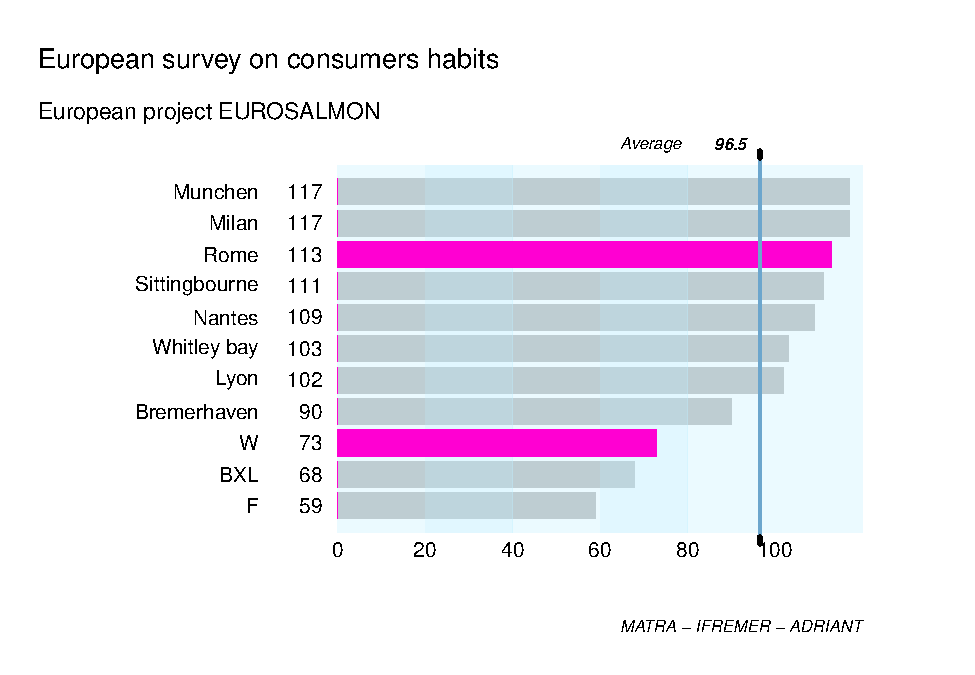
\includegraphics{salmon_files/figure-latex/unnamed-chunk-26-1.pdf}

\hypertarget{understanding-the-consumers-behaviour}{%
\section{Understanding the consumers' behaviour}\label{understanding-the-consumers-behaviour}}

In this part, we're going to play with the questionnaire data. These data are categorical, and you have to use a specific method for these particular data: Multiple Correspondence Analysis (MCA).

\begin{Shaded}
\begin{Highlighting}[]
\FunctionTok{colnames}\NormalTok{(salmon\_hedo\_conso)}
\end{Highlighting}
\end{Shaded}

\begin{verbatim}
##   [1] "IKIDEN"                   "Country"                 
##   [3] "prod1_Fr"                 "prod2_Fr"                
##   [5] "prod3_Fr"                 "prod4_Scot"              
##   [7] "prod5_Ger"                "prod6_Ire"               
##   [9] "prod7_Ire"                "prod8_Ger"               
##  [11] "prod9_Ire"                "prod10_It"               
##  [13] "prod11_Fr"                "prod12_Dk"               
##  [15] "prod13_Ger"               "prod14_Ger"              
##  [17] "prod15_Fr"                "prod16_Ger"              
##  [19] "prod17_Fr"                "prod18_UK"               
##  [21] "prod19_UK"                "prod20_Dk"               
##  [23] "prod21_UK"                "prod22_Fr"               
##  [25] "prod23_Ger"               "prod24_Dk"               
##  [27] "prod25_Bel"               "prod26_UK"               
##  [29] "prod27_Fr"                "prod28_Bel"              
##  [31] "prod29_Scot"              "prod30_Bel"              
##  [33] "Who"                      "Frequence"               
##  [35] "When"                     "Taste"                   
##  [37] "Healthy"                  "Pleasure"                
##  [39] "No.preparation"           "Ways"                    
##  [41] "Guest"                    "Authentic"               
##  [43] "Not.expensive"            "Supermarket"             
##  [45] "Deli"                     "Caterer"                 
##  [47] "Fish.shop"                "Market"                  
##  [49] "Mobile.van"               "Everyday"                
##  [51] "Special"                  "Day.snack"               
##  [53] "Evening.snack"            "Aperitif"                
##  [55] "Starter"                  "Salad"                   
##  [57] "Cooked.meal"              "Sandwich"                
##  [59] "Main"                     "Vegetable"               
##  [61] "Lemon"                    "Bread, butter"           
##  [63] "Lemon, bread, butter"     "Crême fraîche"           
##  [65] "Crême fraîche with herbs" "Fresh cheese"            
##  [67] "Fresh.cheese.with.herbs"  "Shallots"                
##  [69] "Mustard"                  "Butter"                  
##  [71] "Black.pepper"             "Horseradish"             
##  [73] "Scottish"                 "Norwegian"               
##  [75] "Atlantic"                 "Irish"                   
##  [77] "Wild"                     "Do.not.know"             
##  [79] "Colour"                   "Price"                   
##  [81] "Origin"                   "Brand"                   
##  [83] "Advertising"              "Glossiness"              
##  [85] "Packaging"                "Labelling.information"   
##  [87] "Number.slices"            "Weight"                  
##  [89] "Use.by.date"              "Usual.brand"             
##  [91] "Appetising"               "Firm"                    
##  [93] "Regular"                  "Nice.colour"             
##  [95] "Nice.odour"               "Smooth.texture"          
##  [97] "Firm.texture"             "Greasy.mouth"            
##  [99] "Characteristic.taste"     "Not too salty"
\end{verbatim}

\begin{Shaded}
\begin{Highlighting}[]
\NormalTok{res.mca }\OtherTok{\textless{}{-}} \FunctionTok{MCA}\NormalTok{(salmon\_hedo\_conso[,}\DecValTok{33}\SpecialCharTok{:}\DecValTok{100}\NormalTok{],}\AttributeTok{graph=}\NormalTok{F)}
\FunctionTok{plot.MCA}\NormalTok{(res.mca,}\AttributeTok{choix=}\StringTok{"ind"}\NormalTok{,}\AttributeTok{invisible =} \StringTok{"var"}\NormalTok{,}\AttributeTok{label=}\StringTok{"none"}\NormalTok{,}\AttributeTok{graph.type =} \StringTok{"classic"}\NormalTok{)}
\end{Highlighting}
\end{Shaded}

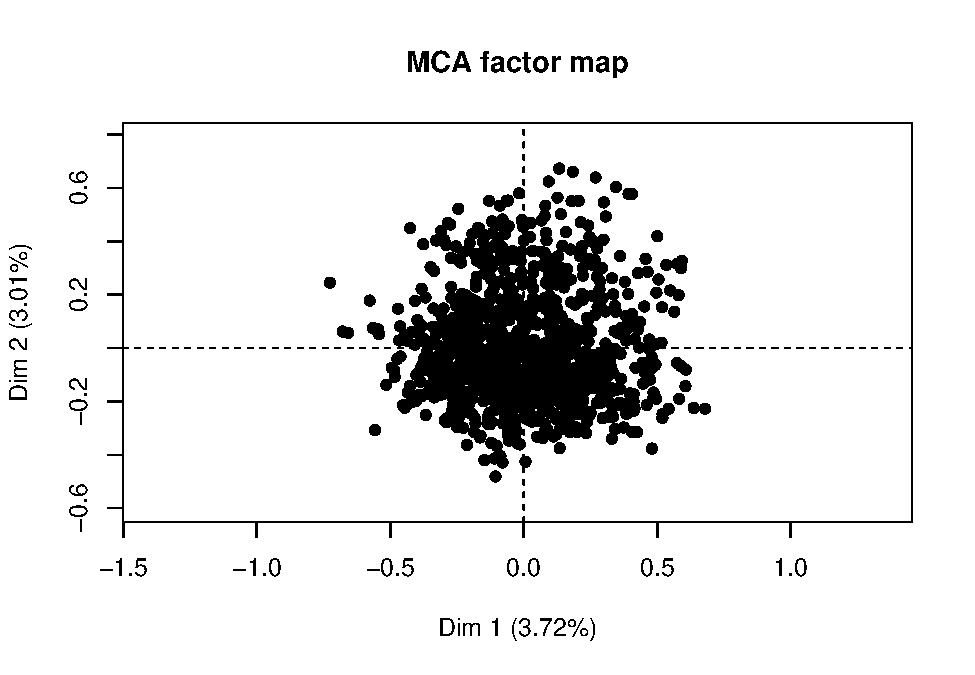
\includegraphics{salmon_files/figure-latex/unnamed-chunk-27-1.pdf}

\begin{Shaded}
\begin{Highlighting}[]
\FunctionTok{plot.MCA}\NormalTok{(res.mca,}\AttributeTok{choix=}\StringTok{"ind"}\NormalTok{,}\AttributeTok{invisible =} \StringTok{"ind"}\NormalTok{)}
\end{Highlighting}
\end{Shaded}

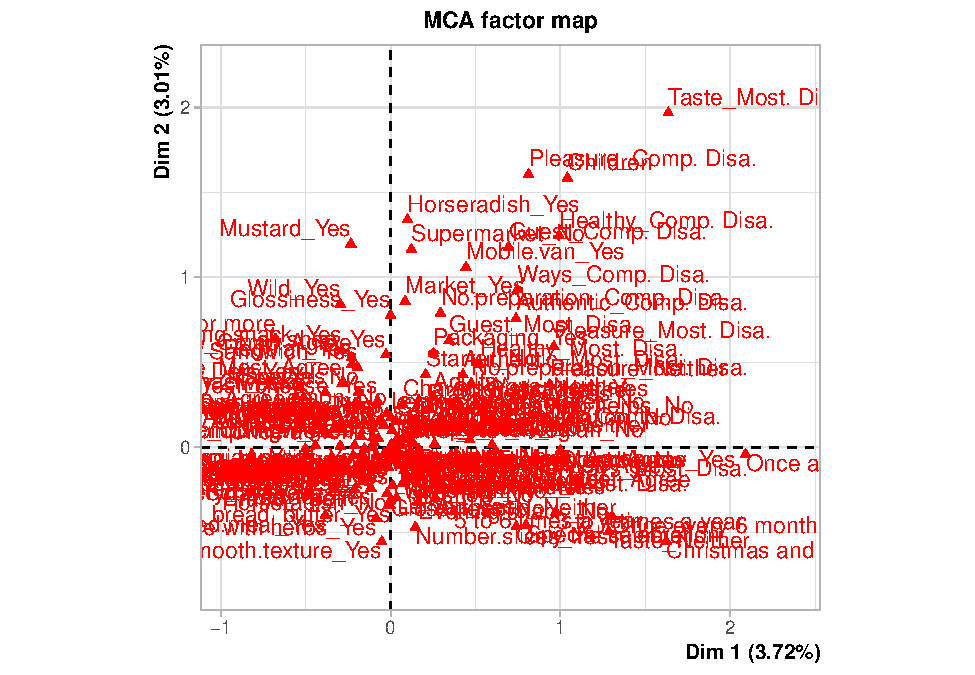
\includegraphics{salmon_files/figure-latex/unnamed-chunk-27-2.pdf}

\begin{Shaded}
\begin{Highlighting}[]
\FunctionTok{plot.MCA}\NormalTok{(res.mca,}\AttributeTok{choix=}\StringTok{"ind"}\NormalTok{,}\AttributeTok{invisible =} \StringTok{"ind"}\NormalTok{,}\AttributeTok{selectMod=}\StringTok{"cos2 10"}\NormalTok{)}
\end{Highlighting}
\end{Shaded}

\begin{verbatim}
## Warning: ggrepel: 7 unlabeled data points (too many overlaps). Consider
## increasing max.overlaps
\end{verbatim}

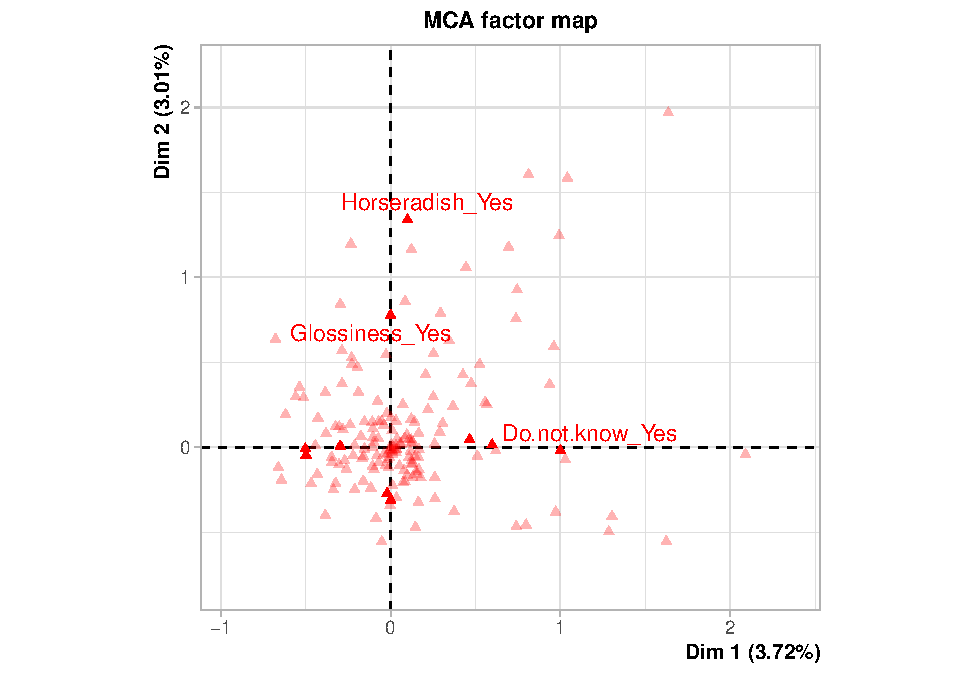
\includegraphics{salmon_files/figure-latex/unnamed-chunk-27-3.pdf}

\textbf{Exercise. }Let's spend some time on these outputs and on the theory behind MCA.

Now, let's run \textbf{MCA} again with some particular inputs. But before that, let's have a look at the variance associated with our dimensions.

\begin{Shaded}
\begin{Highlighting}[]
\NormalTok{res.mca}\SpecialCharTok{$}\NormalTok{eig}
\end{Highlighting}
\end{Shaded}

\begin{verbatim}
##           eigenvalue percentage of variance cumulative percentage of variance
## dim 1   5.473825e-02           3.722201e+00                          3.722201
## dim 2   4.431036e-02           3.013104e+00                          6.735305
## dim 3   4.003557e-02           2.722419e+00                          9.457724
## dim 4   3.392450e-02           2.306866e+00                         11.764590
## dim 5   3.108617e-02           2.113860e+00                         13.878450
## dim 6   2.967338e-02           2.017790e+00                         15.896239
## dim 7   2.855847e-02           1.941976e+00                         17.838216
## dim 8   2.588124e-02           1.759924e+00                         19.598140
## dim 9   2.528128e-02           1.719127e+00                         21.317267
## dim 10  2.450188e-02           1.666128e+00                         22.983394
## dim 11  2.405695e-02           1.635872e+00                         24.619267
## dim 12  2.287132e-02           1.555249e+00                         26.174516
## dim 13  2.266484e-02           1.541209e+00                         27.715725
## dim 14  2.184724e-02           1.485612e+00                         29.201337
## dim 15  2.143759e-02           1.457756e+00                         30.659094
## dim 16  2.102278e-02           1.429549e+00                         32.088643
## dim 17  2.044787e-02           1.390455e+00                         33.479098
## dim 18  1.973262e-02           1.341818e+00                         34.820916
## dim 19  1.964806e-02           1.336068e+00                         36.156984
## dim 20  1.953184e-02           1.328165e+00                         37.485148
## dim 21  1.901586e-02           1.293078e+00                         38.778227
## dim 22  1.879663e-02           1.278171e+00                         40.056398
## dim 23  1.841331e-02           1.252105e+00                         41.308503
## dim 24  1.808677e-02           1.229901e+00                         42.538403
## dim 25  1.799709e-02           1.223802e+00                         43.762205
## dim 26  1.787002e-02           1.215161e+00                         44.977367
## dim 27  1.760494e-02           1.197136e+00                         46.174503
## dim 28  1.748220e-02           1.188789e+00                         47.363292
## dim 29  1.711750e-02           1.163990e+00                         48.527282
## dim 30  1.687421e-02           1.147446e+00                         49.674728
## dim 31  1.656551e-02           1.126455e+00                         50.801183
## dim 32  1.644550e-02           1.118294e+00                         51.919477
## dim 33  1.615074e-02           1.098251e+00                         53.017728
## dim 34  1.597042e-02           1.085988e+00                         54.103716
## dim 35  1.567450e-02           1.065866e+00                         55.169582
## dim 36  1.562135e-02           1.062252e+00                         56.231834
## dim 37  1.528656e-02           1.039486e+00                         57.271320
## dim 38  1.512550e-02           1.028534e+00                         58.299854
## dim 39  1.498150e-02           1.018742e+00                         59.318596
## dim 40  1.483964e-02           1.009096e+00                         60.327692
## dim 41  1.471166e-02           1.000393e+00                         61.328085
## dim 42  1.436120e-02           9.765616e-01                         62.304646
## dim 43  1.412491e-02           9.604939e-01                         63.265140
## dim 44  1.408263e-02           9.576190e-01                         64.222759
## dim 45  1.394252e-02           9.480915e-01                         65.170850
## dim 46  1.381506e-02           9.394244e-01                         66.110275
## dim 47  1.370087e-02           9.316590e-01                         67.041934
## dim 48  1.358617e-02           9.238597e-01                         67.965794
## dim 49  1.346130e-02           9.153686e-01                         68.881162
## dim 50  1.333994e-02           9.071159e-01                         69.788278
## dim 51  1.307056e-02           8.887983e-01                         70.677076
## dim 52  1.294615e-02           8.803382e-01                         71.557414
## dim 53  1.282083e-02           8.718162e-01                         72.429231
## dim 54  1.262218e-02           8.583081e-01                         73.287539
## dim 55  1.249028e-02           8.493392e-01                         74.136878
## dim 56  1.230169e-02           8.365149e-01                         74.973393
## dim 57  1.215842e-02           8.267726e-01                         75.800166
## dim 58  1.207068e-02           8.208064e-01                         76.620972
## dim 59  1.168354e-02           7.944807e-01                         77.415453
## dim 60  1.161892e-02           7.900864e-01                         78.205539
## dim 61  1.130664e-02           7.688518e-01                         78.974391
## dim 62  1.119342e-02           7.611523e-01                         79.735543
## dim 63  1.111680e-02           7.559427e-01                         80.491486
## dim 64  1.092116e-02           7.426388e-01                         81.234125
## dim 65  1.084369e-02           7.373710e-01                         81.971496
## dim 66  1.067418e-02           7.258442e-01                         82.697340
## dim 67  1.034072e-02           7.031693e-01                         83.400509
## dim 68  1.028899e-02           6.996510e-01                         84.100160
## dim 69  1.017623e-02           6.919836e-01                         84.792144
## dim 70  1.001043e-02           6.807096e-01                         85.472853
## dim 71  9.931163e-03           6.753191e-01                         86.148172
## dim 72  9.819269e-03           6.677103e-01                         86.815883
## dim 73  9.678037e-03           6.581065e-01                         87.473989
## dim 74  9.512016e-03           6.468171e-01                         88.120806
## dim 75  9.192120e-03           6.250642e-01                         88.745870
## dim 76  8.990496e-03           6.113537e-01                         89.357224
## dim 77  8.898534e-03           6.051003e-01                         89.962324
## dim 78  8.784312e-03           5.973332e-01                         90.559658
## dim 79  8.658067e-03           5.887486e-01                         91.148406
## dim 80  8.385134e-03           5.701891e-01                         91.718595
## dim 81  8.362101e-03           5.686229e-01                         92.287218
## dim 82  8.224928e-03           5.592951e-01                         92.846513
## dim 83  8.045518e-03           5.470952e-01                         93.393609
## dim 84  7.965330e-03           5.416425e-01                         93.935251
## dim 85  7.684237e-03           5.225281e-01                         94.457779
## dim 86  7.538355e-03           5.126081e-01                         94.970387
## dim 87  7.383017e-03           5.020451e-01                         95.472432
## dim 88  7.252892e-03           4.931967e-01                         95.965629
## dim 89  7.029512e-03           4.780068e-01                         96.443636
## dim 90  6.974460e-03           4.742633e-01                         96.917899
## dim 91  6.646082e-03           4.519336e-01                         97.369833
## dim 92  6.334576e-03           4.307511e-01                         97.800584
## dim 93  6.128442e-03           4.167340e-01                         98.217318
## dim 94  5.857748e-03           3.983269e-01                         98.615645
## dim 95  5.560695e-03           3.781273e-01                         98.993772
## dim 96  4.696508e-03           3.193625e-01                         99.313135
## dim 97  4.314317e-03           2.933735e-01                         99.606508
## dim 98  3.334220e-03           2.267270e-01                         99.833235
## dim 99  2.452426e-03           1.667650e-01                        100.000000
## dim 100 1.016417e-30           6.911637e-29                        100.000000
\end{verbatim}

In the following code, we store the results from the 50 first dimensions, and we get rid of the categories that are not chosen, according to a given threshold.

\begin{Shaded}
\begin{Highlighting}[]
\NormalTok{res.mca }\OtherTok{\textless{}{-}} \FunctionTok{MCA}\NormalTok{(salmon\_hedo\_conso[,}\FunctionTok{c}\NormalTok{(}\DecValTok{2}\NormalTok{,}\DecValTok{33}\SpecialCharTok{:}\DecValTok{100}\NormalTok{)],}\AttributeTok{quali.sup=}\DecValTok{1}\NormalTok{,}\AttributeTok{graph=}\NormalTok{F,}\AttributeTok{ncp=}\DecValTok{50}\NormalTok{,}\AttributeTok{level.ventil=}\FloatTok{0.05}\NormalTok{)}
\end{Highlighting}
\end{Shaded}

\textbf{Exercise. }Let's give some interpretation to the results.

\begin{Shaded}
\begin{Highlighting}[]
\NormalTok{res.dim }\OtherTok{\textless{}{-}} \FunctionTok{dimdesc}\NormalTok{(res.mca)}
\FunctionTok{names}\NormalTok{(res.dim)}
\FunctionTok{names}\NormalTok{(res.dim}\SpecialCharTok{$}\StringTok{\textasciigrave{}}\AttributeTok{Dim 1}\StringTok{\textasciigrave{}}\NormalTok{)}
\NormalTok{res.dim}\SpecialCharTok{$}\StringTok{\textasciigrave{}}\AttributeTok{Dim 1}\StringTok{\textasciigrave{}}\SpecialCharTok{$}\StringTok{"quali"}
\NormalTok{res.dim}\SpecialCharTok{$}\StringTok{\textasciigrave{}}\AttributeTok{Dim 1}\StringTok{\textasciigrave{}}\SpecialCharTok{$}\StringTok{"category"}
\NormalTok{res.dim}\SpecialCharTok{$}\StringTok{\textasciigrave{}}\AttributeTok{Dim 2}\StringTok{\textasciigrave{}}\SpecialCharTok{$}\StringTok{"category"}
\end{Highlighting}
\end{Shaded}

As we said previously, MCA as PCA will reduce the complexity of your data by extracting relevant dimensions. To reduce the complexity from an individual point of view, you have to cluster the individuals.

\begin{Shaded}
\begin{Highlighting}[]
\NormalTok{res.hcpc }\OtherTok{\textless{}{-}} \FunctionTok{HCPC}\NormalTok{(res.mca,}\AttributeTok{nb.clust =} \DecValTok{3}\NormalTok{)}
\end{Highlighting}
\end{Shaded}

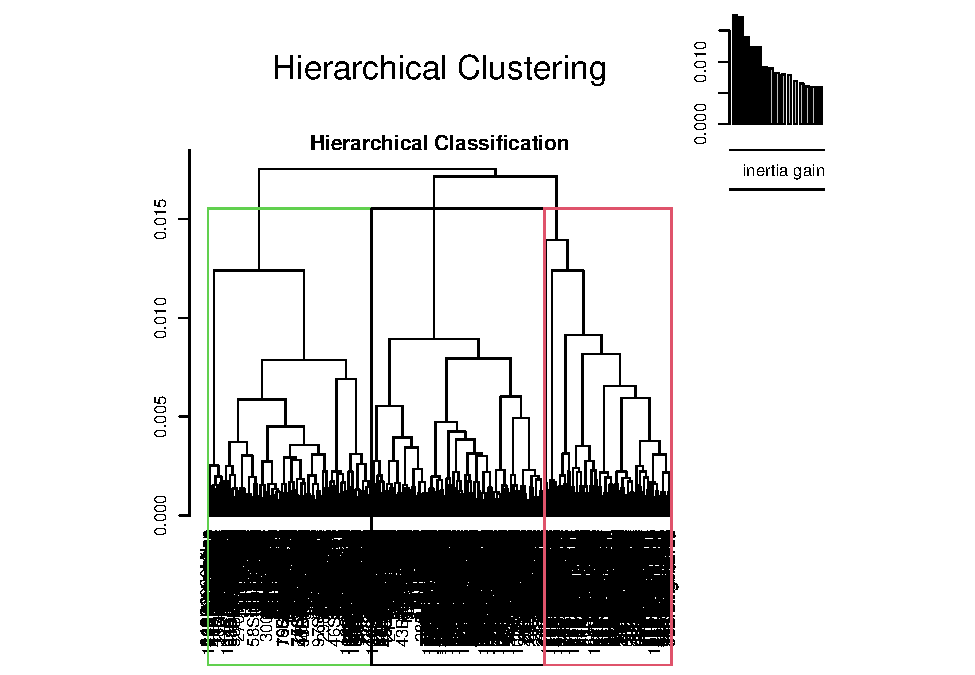
\includegraphics{salmon_files/figure-latex/unnamed-chunk-31-1.pdf} 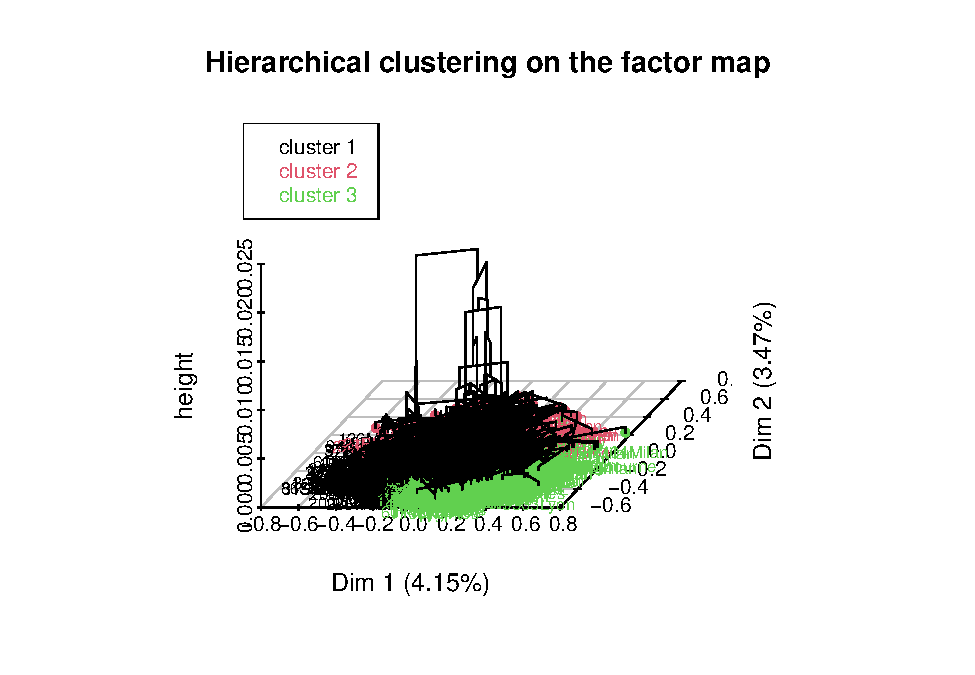
\includegraphics{salmon_files/figure-latex/unnamed-chunk-31-2.pdf} 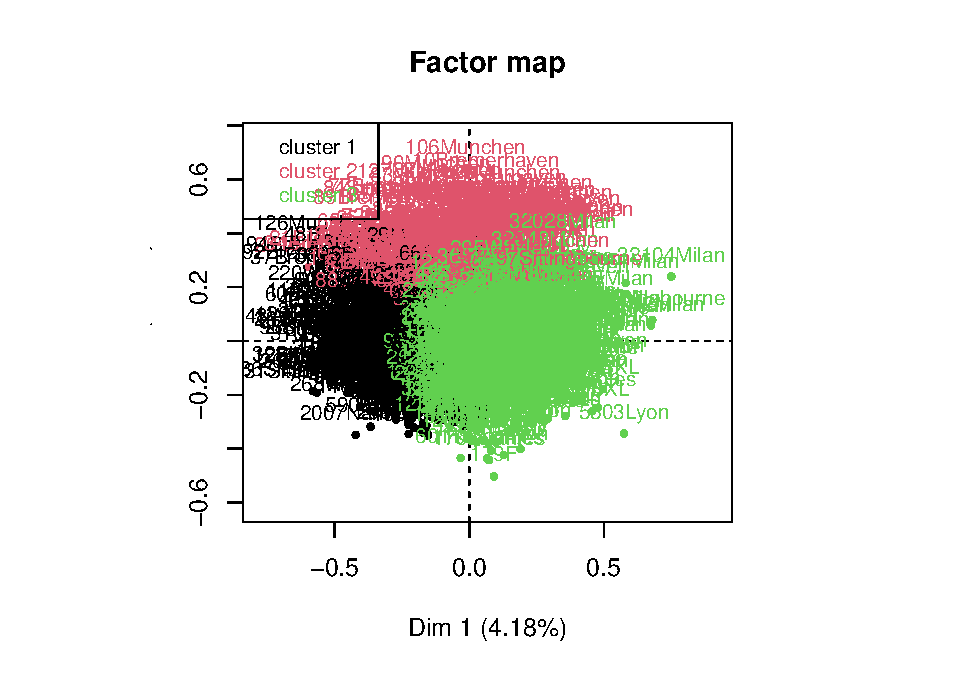
\includegraphics{salmon_files/figure-latex/unnamed-chunk-31-3.pdf}

\textbf{Exercise. }Let's give some interpretation to the results.

\begin{Shaded}
\begin{Highlighting}[]
\FunctionTok{round}\NormalTok{(res.hcpc}\SpecialCharTok{$}\NormalTok{desc.var}\SpecialCharTok{$}\NormalTok{category}\SpecialCharTok{$}\StringTok{\textasciigrave{}}\AttributeTok{1}\StringTok{\textasciigrave{}}\NormalTok{,}\DecValTok{2}\NormalTok{)}
\FunctionTok{round}\NormalTok{(res.hcpc}\SpecialCharTok{$}\NormalTok{desc.var}\SpecialCharTok{$}\NormalTok{category}\SpecialCharTok{$}\StringTok{\textasciigrave{}}\AttributeTok{2}\StringTok{\textasciigrave{}}\NormalTok{,}\DecValTok{2}\NormalTok{)}
\FunctionTok{round}\NormalTok{(res.hcpc}\SpecialCharTok{$}\NormalTok{desc.var}\SpecialCharTok{$}\NormalTok{category}\SpecialCharTok{$}\StringTok{\textasciigrave{}}\AttributeTok{3}\StringTok{\textasciigrave{}}\NormalTok{,}\DecValTok{2}\NormalTok{)}
\end{Highlighting}
\end{Shaded}

\hypertarget{understanding-the-consumers-preferences}{%
\section{Understanding the consumers' preferences}\label{understanding-the-consumers-preferences}}

\textbf{Exercise. }You should be able to do that by yourself using PCA.

\hypertarget{linking-consumers-preferences-and-behaviour}{%
\section{Linking consumers' preferences and behaviour}\label{linking-consumers-preferences-and-behaviour}}

To do so, we're going to import a new dataset.

\begin{Shaded}
\begin{Highlighting}[]
\NormalTok{salmon\_final }\OtherTok{\textless{}{-}} \FunctionTok{read.delim2}\NormalTok{(}\StringTok{"saumon\_final.txt"}\NormalTok{, }\AttributeTok{header=}\ConstantTok{TRUE}\NormalTok{, }\AttributeTok{row.names=}\DecValTok{1}\NormalTok{, }\AttributeTok{comment.char=}\StringTok{"\#"}\NormalTok{,}\AttributeTok{dec=}\StringTok{","}\NormalTok{,}\AttributeTok{stringsAsFactors=}\ConstantTok{TRUE}\NormalTok{)}
\FunctionTok{colnames}\NormalTok{(salmon\_final)}
\end{Highlighting}
\end{Shaded}

\begin{verbatim}
##  [1] "Country"                 "prod1_Fr"               
##  [3] "prod2_Fr"                "prod3_Fr"               
##  [5] "prod4_Scot"              "prod5_Ger"              
##  [7] "prod6_Ire"               "prod7_Ire"              
##  [9] "prod8_Ger"               "prod9_Ire"              
## [11] "prod10_It"               "prod11_Fr"              
## [13] "prod12_Dk"               "prod13_Ger"             
## [15] "prod14_Ger"              "prod15_Fr"              
## [17] "prod16_Ger"              "prod17_Fr"              
## [19] "prod18_UK"               "prod19_UK"              
## [21] "prod20_Dk"               "prod21_UK"              
## [23] "prod22_Fr"               "prod23_Ger"             
## [25] "prod24_Dk"               "prod25_Bel"             
## [27] "prod26_UK"               "prod27_Fr"              
## [29] "prod28_Bel"              "prod29_Scot"            
## [31] "prod30_Bel"              "Who"                    
## [33] "Frequence"               "When"                   
## [35] "Taste"                   "Healthy"                
## [37] "Pleasure"                "No.preparation"         
## [39] "Ways"                    "Guest"                  
## [41] "Authentic"               "Not.expensive"          
## [43] "Supermarket"             "Deli"                   
## [45] "Caterer"                 "Fish.shop"              
## [47] "Market"                  "Mobile.van"             
## [49] "Everyday"                "Special"                
## [51] "Day.snack"               "Evening.snack"          
## [53] "Aperitif"                "Starter"                
## [55] "Salad"                   "Cooked.meal"            
## [57] "Sandwich"                "Main"                   
## [59] "Vegetable"               "Lemon"                  
## [61] "Bread..butter"           "Lemon..bread..butter"   
## [63] "C..fraiche"              "C..fraiche.with.herbs"  
## [65] "Fresh.cheese"            "Fresh.cheese.with.herbs"
## [67] "Shallots"                "Mustard"                
## [69] "Butter"                  "Black.pepper"           
## [71] "Horseradish"             "Scottish"               
## [73] "Norwegian"               "Atlantic"               
## [75] "Irish"                   "Wild"                   
## [77] "Do.not.know"             "Colour"                 
## [79] "Price"                   "Origin"                 
## [81] "Brand"                   "Advertising"            
## [83] "Glossiness"              "Packaging"              
## [85] "Labelling.information"   "Number.slices"          
## [87] "Weight"                  "Use.by.date"            
## [89] "Usual.brand"             "Appetising"             
## [91] "Firm"                    "Regular"                
## [93] "Nice.colour"             "Nice.odour"             
## [95] "Smooth.texture"          "Firm.texture"           
## [97] "Greasy.mouth"            "Characteristic.taste"   
## [99] "Not.too.salty"
\end{verbatim}

\begin{Shaded}
\begin{Highlighting}[]
\FunctionTok{summary}\NormalTok{(salmon\_final)}
\end{Highlighting}
\end{Shaded}

\begin{verbatim}
##           Country       prod1_Fr          prod2_Fr           prod3_Fr      
##  Milan        :117   Min.   :-2.1360   Min.   :-3.72220   Min.   :-2.7302  
##  Munchen      :117   1st Qu.:-0.3792   1st Qu.:-0.68227   1st Qu.:-0.9418  
##  Rome         :113   Median : 0.3375   Median : 0.14975   Median :-0.1079  
##  Sittingbourne:111   Mean   : 0.2449   Mean   : 0.05328   Mean   :-0.1432  
##  Nantes       :109   3rd Qu.: 0.9498   3rd Qu.: 0.85860   3rd Qu.: 0.6805  
##  (Other)      :495   Max.   : 2.9666   Max.   : 2.26040   Max.   : 2.2639  
##  NA's         : 16                                                         
##    prod4_Scot        prod5_Ger         prod6_Ire         prod7_Ire      
##  Min.   :-2.1235   Min.   :-2.5337   Min.   :-2.5977   Min.   :-3.1814  
##  1st Qu.:-0.3402   1st Qu.:-0.4214   1st Qu.:-0.5485   1st Qu.:-0.9107  
##  Median : 0.3216   Median : 0.4385   Median : 0.2509   Median :-0.1588  
##  Mean   : 0.2441   Mean   : 0.2742   Mean   : 0.1209   Mean   :-0.1716  
##  3rd Qu.: 0.9045   3rd Qu.: 1.0171   3rd Qu.: 0.8300   3rd Qu.: 0.5827  
##  Max.   : 3.3236   Max.   : 2.2748   Max.   : 2.3256   Max.   : 2.1494  
##                                                                         
##    prod8_Ger          prod9_Ire         prod10_It         prod11_Fr        
##  Min.   :-2.88000   Min.   :-5.3852   Min.   :-3.1743   Min.   :-3.230300  
##  1st Qu.:-0.85177   1st Qu.:-0.5113   1st Qu.:-1.1188   1st Qu.:-0.755450  
##  Median : 0.08645   Median : 0.2898   Median :-0.3628   Median : 0.082500  
##  Mean   :-0.02674   Mean   : 0.1705   Mean   :-0.3298   Mean   :-0.004231  
##  3rd Qu.: 0.83125   3rd Qu.: 0.9240   3rd Qu.: 0.4482   3rd Qu.: 0.779475  
##  Max.   : 2.47150   Max.   : 2.1506   Max.   : 2.6033   Max.   : 2.221300  
##                                                                            
##    prod12_Dk          prod13_Ger        prod14_Ger          prod15_Fr      
##  Min.   :-3.33710   Min.   :-2.3088   Min.   :-2.268400   Min.   :-2.9948  
##  1st Qu.:-0.80417   1st Qu.:-0.5555   1st Qu.:-0.811625   1st Qu.:-0.7893  
##  Median : 0.11725   Median : 0.2959   Median : 0.068150   Median : 0.0400  
##  Mean   : 0.02101   Mean   : 0.1762   Mean   :-0.004349   Mean   :-0.0387  
##  3rd Qu.: 0.86582   3rd Qu.: 0.9180   3rd Qu.: 0.776725   3rd Qu.: 0.7484  
##  Max.   : 2.23290   Max.   : 2.5355   Max.   : 2.171200   Max.   : 2.9253  
##                                                                            
##    prod16_Ger        prod17_Fr         prod18_UK          prod19_UK       
##  Min.   :-2.8800   Min.   :-3.1593   Min.   :-4.76160   Min.   :-3.02240  
##  1st Qu.:-1.0514   1st Qu.:-0.5131   1st Qu.:-1.05927   1st Qu.:-0.96270  
##  Median :-0.1039   Median : 0.2937   Median :-0.08125   Median : 0.03750  
##  Mean   :-0.1459   Mean   : 0.1955   Mean   :-0.11816   Mean   :-0.05406  
##  3rd Qu.: 0.7220   3rd Qu.: 0.9249   3rd Qu.: 0.80950   3rd Qu.: 0.84418  
##  Max.   : 2.5916   Max.   : 2.2967   Max.   : 2.40620   Max.   : 2.46320  
##                                                                           
##    prod20_Dk         prod21_UK         prod22_Fr         prod23_Ger     
##  Min.   :-2.9866   Min.   :-3.9939   Min.   :-2.5573   Min.   :-2.7796  
##  1st Qu.:-1.0533   1st Qu.:-1.3312   1st Qu.:-0.3749   1st Qu.:-0.5266  
##  Median :-0.2591   Median :-0.6193   Median : 0.4213   Median : 0.2942  
##  Mean   :-0.2464   Mean   :-0.4841   Mean   : 0.2813   Mean   : 0.2050  
##  3rd Qu.: 0.5691   3rd Qu.: 0.3917   3rd Qu.: 0.9916   3rd Qu.: 0.9395  
##  Max.   : 2.2533   Max.   : 2.5982   Max.   : 2.9192   Max.   : 2.2837  
##                                                                         
##    prod24_Dk         prod25_Bel        prod26_UK           prod27_Fr      
##  Min.   :-2.9200   Min.   :-3.7989   Min.   :-3.246900   Min.   :-3.4338  
##  1st Qu.:-0.9318   1st Qu.:-1.0870   1st Qu.:-0.775475   1st Qu.:-0.5243  
##  Median :-0.1290   Median :-0.2250   Median : 0.031850   Median : 0.2656  
##  Mean   :-0.1660   Mean   :-0.2191   Mean   : 0.006847   Mean   : 0.1487  
##  3rd Qu.: 0.5792   3rd Qu.: 0.6603   3rd Qu.: 0.836275   3rd Qu.: 0.9037  
##  Max.   : 2.1106   Max.   : 2.6322   Max.   : 2.335100   Max.   : 2.1495  
##                                                                           
##    prod28_Bel        prod29_Scot         prod30_Bel             Who     
##  Min.   :-3.86570   Min.   :-2.85220   Min.   :-3.09880   Adults  :483  
##  1st Qu.:-0.90548   1st Qu.:-0.67820   1st Qu.:-0.80875   Both    :578  
##  Median :-0.06030   Median : 0.14665   Median : 0.07245   Children:  1  
##  Mean   :-0.07935   Mean   : 0.07244   Mean   : 0.01685   NA's    : 16  
##  3rd Qu.: 0.78902   3rd Qu.: 0.84535   3rd Qu.: 0.90955                 
##  Max.   : 2.26810   Max.   : 2.48480   Max.   : 3.45930                 
##                                                                         
##                Frequence                    When             Taste    
##  Once a month       :364   All year round     :785   Comp. Agree:809  
##  Once every 2 weeks :245   Christmas and NY   : 21   Most. Agree:232  
##  5 to 6 times a year:235   Only the summer    : 22   Most. Disa.:  3  
##  Once a week or more: 96   Only the winter    : 74   Neither    : 18  
##  3 to 4 times a year: 81   Special celebration:160   NA's       : 16  
##  (Other)            : 41   NA's               : 16                    
##  NA's               : 16                                              
##         Healthy           Pleasure       No.preparation          Ways    
##  Comp. Agree:240   Comp. Agree:509   Comp. Agree:367    Comp. Agree:467  
##  Comp. Disa.: 26   Comp. Disa.: 16   Comp. Disa.: 50    Comp. Disa.: 11  
##  Most. Agree:345   Most. Agree:386   Most. Agree:330    Most. Agree:382  
##  Most. Disa.: 60   Most. Disa.: 27   Most. Disa.: 91    Most. Disa.: 49  
##  Neither    :391   Neither    :124   Neither    :224    Neither    :153  
##  NA's       : 16   NA's       : 16   NA's       : 16    NA's       : 16  
##                                                                          
##          Guest           Authentic       Not.expensive Supermarket   Deli    
##  Comp. Agree:639   Comp. Agree:200   Comp. Agree: 43   No  :101    No  :865  
##  Comp. Disa.: 16   Comp. Disa.: 75   Comp. Disa.:136   Yes :961    Yes :197  
##  Most. Agree:290   Most. Agree:291   Most. Agree:168   NA's: 16    NA's: 16  
##  Most. Disa.: 15   Most. Disa.:108   Most. Disa.:361                         
##  Neither    :102   Neither    :388   Neither    :354                         
##  NA's       : 16   NA's       : 16   NA's       : 16                         
##                                                                              
##  Caterer    Fish.shop   Market    Mobile.van  Everyday   Special    Day.snack 
##  No  :970   No  :750   No  :989   No  :1042   No  :642   No  :360   No  :888  
##  Yes : 92   Yes :312   Yes : 73   Yes :  20   Yes :420   Yes :702   Yes :174  
##  NA's: 16   NA's: 16   NA's: 16   NA's:  16   NA's: 16   NA's: 16   NA's: 16  
##                                                                               
##                                                                               
##                                                                               
##                                                                               
##  Evening.snack Aperitif   Starter     Salad     Cooked.meal Sandwich  
##  No  :676      No  :398   No  :383   No  :787   No  :776    No  :740  
##  Yes :386      Yes :664   Yes :679   Yes :275   Yes :286    Yes :322  
##  NA's: 16      NA's: 16   NA's: 16   NA's: 16   NA's: 16    NA's: 16  
##                                                                       
##                                                                       
##                                                                       
##                                                                       
##    Main     Vegetable   Lemon     Bread..butter Lemon..bread..butter C..fraiche
##  No  :806   No  :720   No  :640   No  :484      No  :706             No  :890  
##  Yes :256   Yes :342   Yes :422   Yes :578      Yes :356             Yes :172  
##  NA's: 16   NA's: 16   NA's: 16   NA's: 16      NA's: 16             NA's: 16  
##                                                                                
##                                                                                
##                                                                                
##                                                                                
##  C..fraiche.with.herbs Fresh.cheese Fresh.cheese.with.herbs Shallots  
##  No  :777              No  :922     No  :919                No  :859  
##  Yes :285              Yes :140     Yes :143                Yes :203  
##  NA's: 16              NA's: 16     NA's: 16                NA's: 16  
##                                                                       
##                                                                       
##                                                                       
##                                                                       
##  Mustard      Butter    Black.pepper Horseradish Scottish   Norwegian 
##  No  :1051   No  :973   No  :906     No  :882    No  :498   No  :485  
##  Yes :  11   Yes : 89   Yes :156     Yes :180    Yes :564   Yes :577  
##  NA's:  16   NA's: 16   NA's: 16     NA's: 16    NA's: 16   NA's: 16  
##                                                                       
##                                                                       
##                                                                       
##                                                                       
##  Atlantic    Irish       Wild     Do.not.know  Colour     Price      Origin   
##  No  :814   No  :897   No  :851   No  :819    No  :244   No  :391   No  :549  
##  Yes :248   Yes :165   Yes :211   Yes :243    Yes :818   Yes :671   Yes :513  
##  NA's: 16   NA's: 16   NA's: 16   NA's: 16    NA's: 16   NA's: 16   NA's: 16  
##                                                                               
##                                                                               
##                                                                               
##                                                                               
##   Brand     Advertising Glossiness Packaging  Labelling.information
##  No  :827   No  :1022   No  :758   No  :981   No  :650             
##  Yes :235   Yes :  40   Yes :304   Yes : 81   Yes :412             
##  NA's: 16   NA's:  16   NA's: 16   NA's: 16   NA's: 16             
##                                                                    
##                                                                    
##                                                                    
##                                                                    
##  Number.slices  Weight    Use.by.date Usual.brand Appetising   Firm    
##  No  :833      No  :892   No  :521    No  :967    No  :588   No  :903  
##  Yes :229      Yes :170   Yes :541    Yes : 95    Yes :474   Yes :159  
##  NA's: 16      NA's: 16   NA's: 16    NA's: 16    NA's: 16   NA's: 16  
##                                                                        
##                                                                        
##                                                                        
##                                                                        
##  Regular     Nice.colour Nice.odour Smooth.texture Firm.texture Greasy.mouth
##  No  :1016   No  :522    No  :611   No  :905       No  :831     No  :649    
##  Yes :  46   Yes :540    Yes :451   Yes :157       Yes :231     Yes :413    
##  NA's:  16   NA's: 16    NA's: 16   NA's: 16       NA's: 16     NA's: 16    
##                                                                             
##                                                                             
##                                                                             
##                                                                             
##  Characteristic.taste Not.too.salty
##  No  :738             No  :671     
##  Yes :324             Yes :391     
##  NA's: 16             NA's: 16     
##                                    
##                                    
##                                    
## 
\end{verbatim}

\begin{Shaded}
\begin{Highlighting}[]
\NormalTok{salmon\_final[}\DecValTok{1063}\SpecialCharTok{:}\DecValTok{1078}\NormalTok{,}\DecValTok{1}\SpecialCharTok{:}\DecValTok{33}\NormalTok{]}
\end{Highlighting}
\end{Shaded}

\begin{verbatim}
##                    Country prod1_Fr prod2_Fr prod3_Fr prod4_Scot prod5_Ger
## water                 <NA>  -0.8644  -1.1476  -0.4172    -0.8147   -1.6991
## lipid                 <NA>   1.1375   0.7036   0.3378    -0.0961    0.0366
## TVBN                  <NA>  -0.7629   0.2357   0.4354    -0.5632   -0.7629
## TMA                   <NA>  -0.8717   0.3204   1.2144    -0.8717   -0.8717
## salt                  <NA>  -0.1471   0.1626   0.3174     0.3174    2.1752
## phenol                <NA>  -0.3776   0.0112   0.4001    -0.4554   -0.3776
## pH                    <NA>   1.5412   1.2098   0.3812     0.2154   -0.2817
## total viable count    <NA>   0.1112   0.4302   0.8225    -0.2432   -1.5584
## lactic flora          <NA>   0.6665  -0.4514   0.8725    -1.5861   -1.5861
## lactobacilli          <NA>   1.1382   0.1290   0.4088    -1.0624   -1.0624
## brochothrix           <NA>   0.5461  -0.7559   0.6465    -0.7559   -0.7559
## yeast                 <NA>   0.7729   1.2034   0.2875    -1.0340   -1.0340
## enterobacteriaceae    <NA>   0.8314   0.5998   0.2524    -1.5793   -0.9582
## L                     <NA>   0.9917   0.8542  -0.8548     0.3020   -1.3485
## a                     <NA>  -0.6467   0.5297   0.3927     1.7439    0.7341
## b                     <NA>  -0.4567   0.9551   0.2813     3.3236    0.5485
##                    prod6_Ire prod7_Ire prod8_Ger prod9_Ire prod10_It prod11_Fr
## water                -0.9886   -1.5848    0.3380    1.9081    0.1095    1.4659
## lipid                 0.9653    1.2809    0.0940   -0.2969   -2.1795   -1.2830
## TVBN                 -0.7629   -0.3635   -0.9626   -1.1623    0.8348   -0.7629
## TMA                  -0.8717   -0.8717   -0.5737   -0.8717    0.0224   -0.2757
## salt                  0.0077    0.0077   -2.0049    1.4011    0.9366   -0.4567
## phenol                0.6594   -0.1702    1.1260    1.4631    0.9964   -0.9350
## pH                    1.0441    0.8783   -1.1104    0.5469    0.3812   -1.7733
## total viable count   -2.5977   -0.9336   -0.2561   -1.1271    0.2176    0.8505
## lactic flora         -1.5861   -0.0449    0.4294   -1.5861    1.5327    0.5524
## lactobacilli         -1.0624    0.3686    0.6069   -1.0624    1.9639    0.9344
## brochothrix          -0.7559   -0.7559   -0.7559   -0.7559    1.9004   -0.7559
## yeast                -1.0340   -1.0340    0.4282   -1.0340    0.7852    2.1072
## enterobacteriaceae   -1.5793   -0.6424   -0.6634   -0.5266    0.8372    1.4683
## L                    -0.4322   -0.4737   -1.0916    0.0550   -1.8353    0.2448
## a                     0.4016    1.2366    0.6655   -0.3624   -1.0433   -0.5423
## b                     0.4278    1.6822    0.9331   -0.6856   -0.5130   -0.0307
##                    prod12_Dk prod13_Ger prod14_Ger prod15_Fr prod16_Ger
## water                 1.3615     0.1939    -0.1787    0.3976     1.5752
## lipid                -0.3005    -0.3722     1.6072    0.5135    -0.9711
## TVBN                 -0.7629     0.2357    -1.1623   -0.9626    -0.7629
## TMA                  -0.5737     0.6184    -0.8717   -0.7346    -0.2757
## salt                 -0.3793    -0.7663     0.3174    0.3948     0.1626
## phenol                0.3223    -1.1036    -0.4554   -0.5591    -0.5980
## pH                    0.8783     0.5469    -0.9446   -0.2817    -0.2817
## total viable count    0.3222     0.8076    -0.8553   -0.1907    -0.2814
## lactic flora          0.8725     0.0282    -0.4082   -0.2986     0.5306
## lactobacilli          1.2442    -1.0624    -1.0624   -1.0624    -1.0624
## brochothrix          -0.7559     0.9831    -0.7559   -0.7559    -0.7559
## yeast                 1.2038    -1.0340    -1.0340   -1.0340     0.4980
## enterobacteriaceae    0.0419     0.9735    -0.9582    1.0419     0.0419
## L                     0.3527     0.5279     1.3714    0.9614     0.3384
## a                    -0.4328     0.4921    -0.0805   -0.2456     0.2588
## b                    -1.5026     0.2601    -0.6433   -0.7466    -0.5323
##                    prod17_Fr prod18_UK prod19_UK prod20_Dk prod21_UK prod22_Fr
## water                -0.3228   -0.5563    1.1131   -0.3675   -1.2072   -0.9985
## lipid                -0.5623    0.3665   -2.4628    1.6251    0.5709    0.5529
## TVBN                 -0.3635    2.0330    1.2342   -0.7629    0.8348    1.4339
## TMA                  -0.8717    2.1085    0.3204   -0.8717    0.3204    1.2144
## salt                  1.5559   -1.0760    0.0077   -0.1471   -0.6115   -0.6889
## phenol               -0.6628    1.0483    1.4890    0.0631   -1.2073    0.0631
## pH                   -1.4418   -0.1160    0.7126   -1.2761   -1.4418   -0.4475
## total viable count   -0.3769    0.6098    0.9992   -0.8152    1.0168    0.6157
## lactic flora         -0.4776    0.8165    1.2062   -0.1654    0.3479    0.8681
## lactobacilli         -1.0624   -1.0624    1.1989    0.2839    0.4541    1.0535
## brochothrix          -0.7559    0.4217    2.4632   -0.7559    1.3957    1.1371
## yeast                -1.0340    0.0682    0.2875    0.9324    0.2341    0.5504
## enterobacteriaceae   -0.6266    0.0216    1.5470   -1.5793    0.0109    0.5577
## L                     0.1846   -0.7728   -0.2587    1.5224    2.5982    0.1901
## a                     0.3111    0.7864    0.2626   -1.3598   -3.9939   -0.0805
## b                     0.2349    0.2931    0.8976   -1.3411   -1.8277    0.3227
##                    prod23_Ger prod24_Dk prod25_Bel prod26_UK prod27_Fr
## water                  2.0273    0.4821     0.4622    0.7554   -0.9240
## lipid                 -1.5341    0.4310    -0.0853   -1.2472    0.3665
## TVBN                  -0.3635   -0.3635     2.6322    0.4354   -0.0439
## TMA                   -0.8717   -0.2757     2.4065    0.6184   -0.1892
## salt                   0.9366   -0.9212    -1.3856   -0.6115    0.0077
## phenol                -0.2221   -0.6369    -0.8443   -1.1813   -0.9739
## pH                    -0.4475    1.3755    -1.2761    2.0384    1.0441
## total viable count    -0.0665    0.4494     1.0223    1.0932    0.3376
## lactic flora          -1.5861   -1.5861     0.8165    0.8362    0.7697
## lactobacilli          -1.0624   -1.0624     1.2312    0.0909    0.5204
## brochothrix           -0.7559   -0.7559    -0.7559    0.9443    1.7156
## yeast                 -1.0340   -1.0340     0.2875   -1.0340    1.9679
## enterobacteriaceae    -1.5793    0.0508    -0.1055    1.4803    1.6472
## L                      1.0328    0.5514    -1.6298   -0.8136   -0.3829
## a                     -0.3553   -0.5153     0.7578    0.5383    0.3803
## b                     -0.4847   -1.4920     0.4104   -0.0762   -0.0363
##                    prod28_Bel prod29_Scot prod30_Bel  Who Frequence
## water                 -0.0048     -0.1439     0.0300 <NA>      <NA>
## lipid                  0.5781     -0.4439     0.6677 <NA>      <NA>
## TVBN                   1.8333     -0.7629     0.2357 <NA>      <NA>
## TMA                    2.1085     -0.8717     1.2144 <NA>      <NA>
## salt                  -1.3856      2.4848    -0.6115 <NA>      <NA>
## phenol                -0.7406      0.4001     3.4593 <NA>      <NA>
## pH                     0.0497     -1.1104    -0.6132 <NA>      <NA>
## total viable count     1.1384     -2.5977     1.0558 <NA>      <NA>
## lactic flora           0.8491     -1.5861     0.9539 <NA>      <NA>
## lactobacilli           1.2539     -1.0624     0.9302 <NA>      <NA>
## brochothrix            0.5758     -0.7559     0.8767 <NA>      <NA>
## yeast                  1.1315     -1.0340     0.6964 <NA>      <NA>
## enterobacteriaceae     0.6682     -1.5793     0.3051 <NA>      <NA>
## L                     -1.0399     -1.2488     0.1036 <NA>      <NA>
## a                      0.4114      0.6412    -0.8857 <NA>      <NA>
## b                      0.2132      0.1780    -0.5929 <NA>      <NA>
\end{verbatim}

\textbf{Exercise. }Let's run the following code and comment.

\begin{Shaded}
\begin{Highlighting}[]
\NormalTok{res\_final }\OtherTok{\textless{}{-}} \FunctionTok{PCA}\NormalTok{(salmon\_final,}\AttributeTok{ind.sup =} \DecValTok{1063}\SpecialCharTok{:}\DecValTok{1078}\NormalTok{,}\AttributeTok{quali.sup=}\FunctionTok{c}\NormalTok{(}\DecValTok{1}\NormalTok{,}\DecValTok{32}\SpecialCharTok{:}\DecValTok{99}\NormalTok{),}\AttributeTok{graph =}\NormalTok{ F)}
\FunctionTok{plot.PCA}\NormalTok{(res\_final,}\AttributeTok{choix=}\StringTok{"ind"}\NormalTok{,}\AttributeTok{invisible =} \FunctionTok{c}\NormalTok{(}\StringTok{"ind"}\NormalTok{,}\StringTok{"quali"}\NormalTok{))}
\FunctionTok{plot.PCA}\NormalTok{(res\_final,}\AttributeTok{choix=}\StringTok{"var"}\NormalTok{)}

\NormalTok{res.dim }\OtherTok{\textless{}{-}} \FunctionTok{dimdesc}\NormalTok{(res\_final)}
\NormalTok{res.dim}\SpecialCharTok{$}\NormalTok{Dim}\FloatTok{.1}\SpecialCharTok{$}\NormalTok{quanti}
\NormalTok{res.dim}\SpecialCharTok{$}\NormalTok{Dim}\FloatTok{.1}\SpecialCharTok{$}\NormalTok{quali}

\NormalTok{cluster\_final }\OtherTok{\textless{}{-}} \FunctionTok{HCPC}\NormalTok{(res\_final)}
\NormalTok{cluster\_final}\SpecialCharTok{$}\NormalTok{desc.var}\SpecialCharTok{$}\NormalTok{category}\SpecialCharTok{$}\StringTok{\textasciigrave{}}\AttributeTok{1}\StringTok{\textasciigrave{}}
\NormalTok{cluster\_final}\SpecialCharTok{$}\NormalTok{desc.var}\SpecialCharTok{$}\NormalTok{category}\SpecialCharTok{$}\StringTok{\textasciigrave{}}\AttributeTok{3}\StringTok{\textasciigrave{}}
\end{Highlighting}
\end{Shaded}

Now, it's your turn to work and to interpret.

\begin{figure}

{\centering 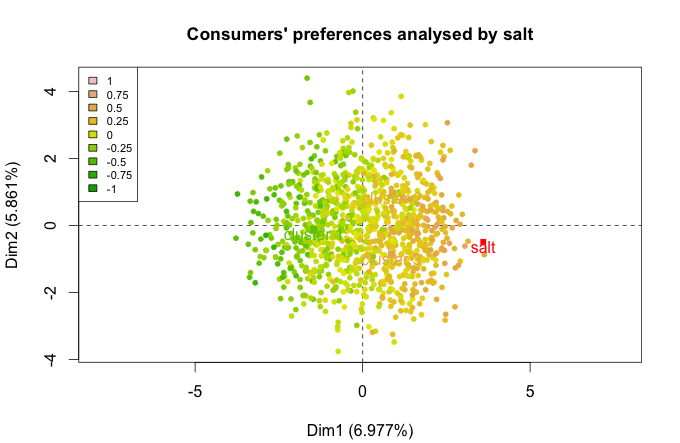
\includegraphics[width=9.44in]{images/salt} 

}

\caption{Consumers according to the variable salt}\label{fig:salt}
\end{figure}

  \bibliography{book.bib,packages.bib}

\end{document}
